\chapter{Experiment}

\section{Operational Principles of Time Projection Chambers}


\begin{figure}
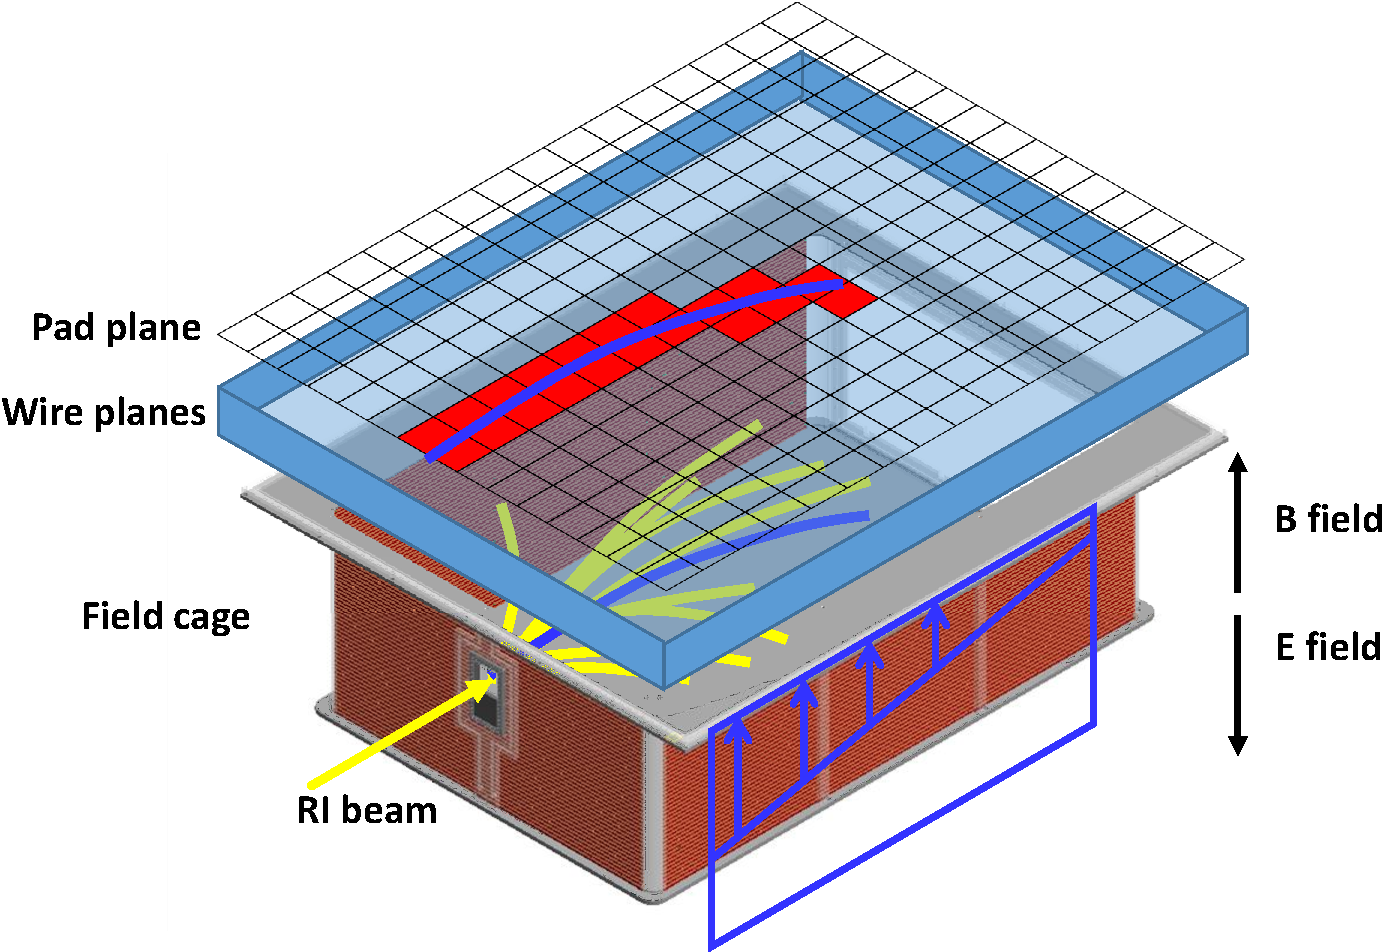
\includegraphics[width=\textwidth]{tpcPrinciple.pdf}
\label{fig:tpcPrinciple}
\caption{Operation principle of the TPC}
\end{figure}
%explain in breif the basics of a time projection chamber 
Time projection chambers are a class of detectors which reconstruct charged particles in all 3-dimensions. Here we will outline the physical principles involved in the TPC measurement and discuss the particular details of the TPC used in this thesis. Inside of at TPC the detector gas is housed in a field cage, which also sets up a constant electric field. As charged particles pass through the gas, electron-ion pairs from neutral gas molecules by passing tracks; the electrons are accelerated opposite to the electric field and the ions move in the opposite direction. Since the mean free path of the electrons inside the gas is very small, they quickly collide with other gas molecules, slowing down the electron, which is then accelerated again repeating the cycle. This microscopic behavior manifests into a constant drift velocity when averaged over several gas collisions. These electrons drift up towards a set of wire planes eventually reaching a set of high voltage anode wires where they accelerate under the high electric field, liberating more electron-ion pairs from the gas creating an avalanche. The avalanche electrons finally terminate either on the anode wire or the grounded pad readout plane,  while the ions from the avalanche move slowly away from the anode wires; creating a large signal which is distributed over the pad-plane where the charge and time information of the signal is measured by the  electronics. 

Two of the 3 coordinates are determined from the charge distribution on the pad plane. The third dimension comes from projecting the electrons back in time, utilizing the known constant drift velocity $v_d$; the distance the electron has traveled , $d$, -- along the electric field direction-- is calculated as $d = v_d \cdot t$, where $t$ is the time it took for the electrons to reach the electronics. The radius of curvature is related to the magnetic rigidity, and therefore the momentum of each track. The energy loss  deposited ($\langle dE/dx\rangle$) is measured by the segmented charge sensitive pads on the pad-plane, which are connected to the readout electronics. Particle identification is achieved through since unique particles exist on unique rigidity and $\langle dE/dx\rangle$  lines, which will be discussed in latter sections. In this chapter we will discuss in more detail the process described above in the context of the specific TPC used in this thesis. 

\section{S$\pi$RIT TPC Overview}
%Add Overview image with labels

\begin{figure}[!htb]
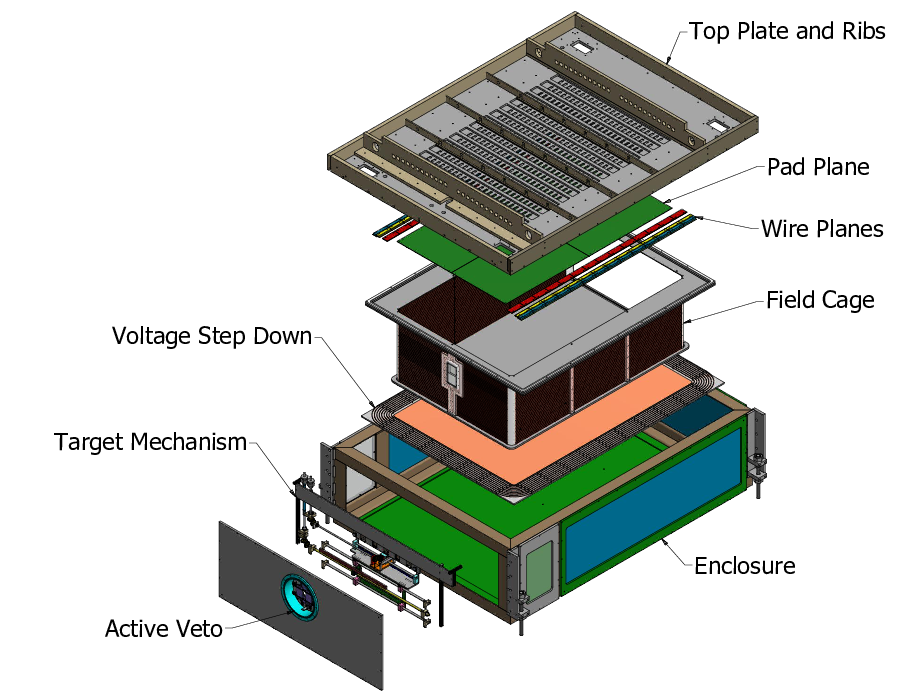
\includegraphics[width=\textwidth]{exploded.png}
\caption{Overview of the \spirit TPC}
\label{fig:tpcExplode}
\end{figure}


The Samurai Pion-Reconstruction and Ion Tracker Time Projection Chamber (\spirit TPC) is a multi-wire proportional counter developed to measure pions and other light charge particles resulting from radioactive heavy ion collisions in fixed target experiments.  The TPC is built on an aluminum angle iron skeleton with thin aluminum sheet walls all around, in order to minimize neutron scattering and to allow for light charged particles to reach auxilliary detectors on the sides and downstream of the TPC. The \spirit TPC was developed to fit inside the SAMURAI dipole magnet used at the Rare Isotope Beam Factory (RIBF) at RIKEN in Wako-shi, Japan \cite{riken}; the dipole gap limited the vertical space of the TPC to around \SI{75}{\centi\metre}. More detail and specifications of the SAMURAI dipole magnet are given in \cite{samurai}. 

A target mechanism allowed for up to 5 fixed targets to be mounted at anytime, with the ability to change targets on the outside of the TPC. The field cage contained the detector gas and set up the constant electric field, which was mounted to a large aluminum top plate, though electrically isolated by a lexan top perimeter ring with o-rings to provide as gas seal. The pad plane and wire plane structures are also mounted to the inside face of the top plate with the electronics being mounted on the outside face of the top plate; several aluminum ribs were also mounted to provide extra rigidity to the top plate, keeping it flat to within \SI{150}{\micro\metre}, as measured by a laser \cite{jon}. Holes on the top plate allowed for the readout of the individual charge sensitive pads on the pad plane, through surface mount pads which were connected through short cables to the electronics. The exploded drawing shown in Fig.~\ref{fig:tpcExplode} pictures all of the major internal components of the  of the \spirit TPC


\begin{table*}\centering
\ra{1.3}
\begin{tabular}{@{}rr@{}}\toprule 
\multicolumn{2}{c}{\spirit TPC Overview} \\
 \midrule
Pad plane area & 1.3 m x .9 m\\
Pad size       & 1.2 cm x .8 cm \\
Number of pads & 12096 (112 x 108) \\
Gas composition& 90\% Ar + 10\% CH${}_4$ (1 atm)  \\
Multiplicity limit & 200  \\
dE/dx range        & Z=1-3, $\pi$, p, d, t, He, Li \\
Drift length       & 50 cm \\
\bottomrule
\end{tabular}
\caption{An overview of the properties of the \spirit TPC}
\label{tb:spiritoverview}
\end{table*}


\subsection{Enclosure}
The skeleton of the enclosure is composed of a rigid aluminum angle-iron frame. All walls are constructed of a aluminum frame with thin sheet metal. All materials were made to be as thin to allow charged particles and neutrons to exit the TPC without scattering too much. This allows for a trigger to be created by placing detectors on the sides and downstream of the TPC. The enclosure itself is made to be gas tight with respects to the outside and the field cage. This is to allow for the possibility to run a different gas inside the enclosure than the field cage. Although, in this set of experiments we ran the same gas in the field cage and enclosure volume. 

\subsection{Field Cage}

The field cage contains the detector gas and sets up a uniform electric field in which electrons can drift upwards toward the anode wires. It was designed to hang from the top plate and therefore needed to be of a lightweight construction. The materials needed to be thin to allow for light charged particle and neutrons to pass through without significant scattering for ancillary detectors. 

\begin{figure}[!htb]
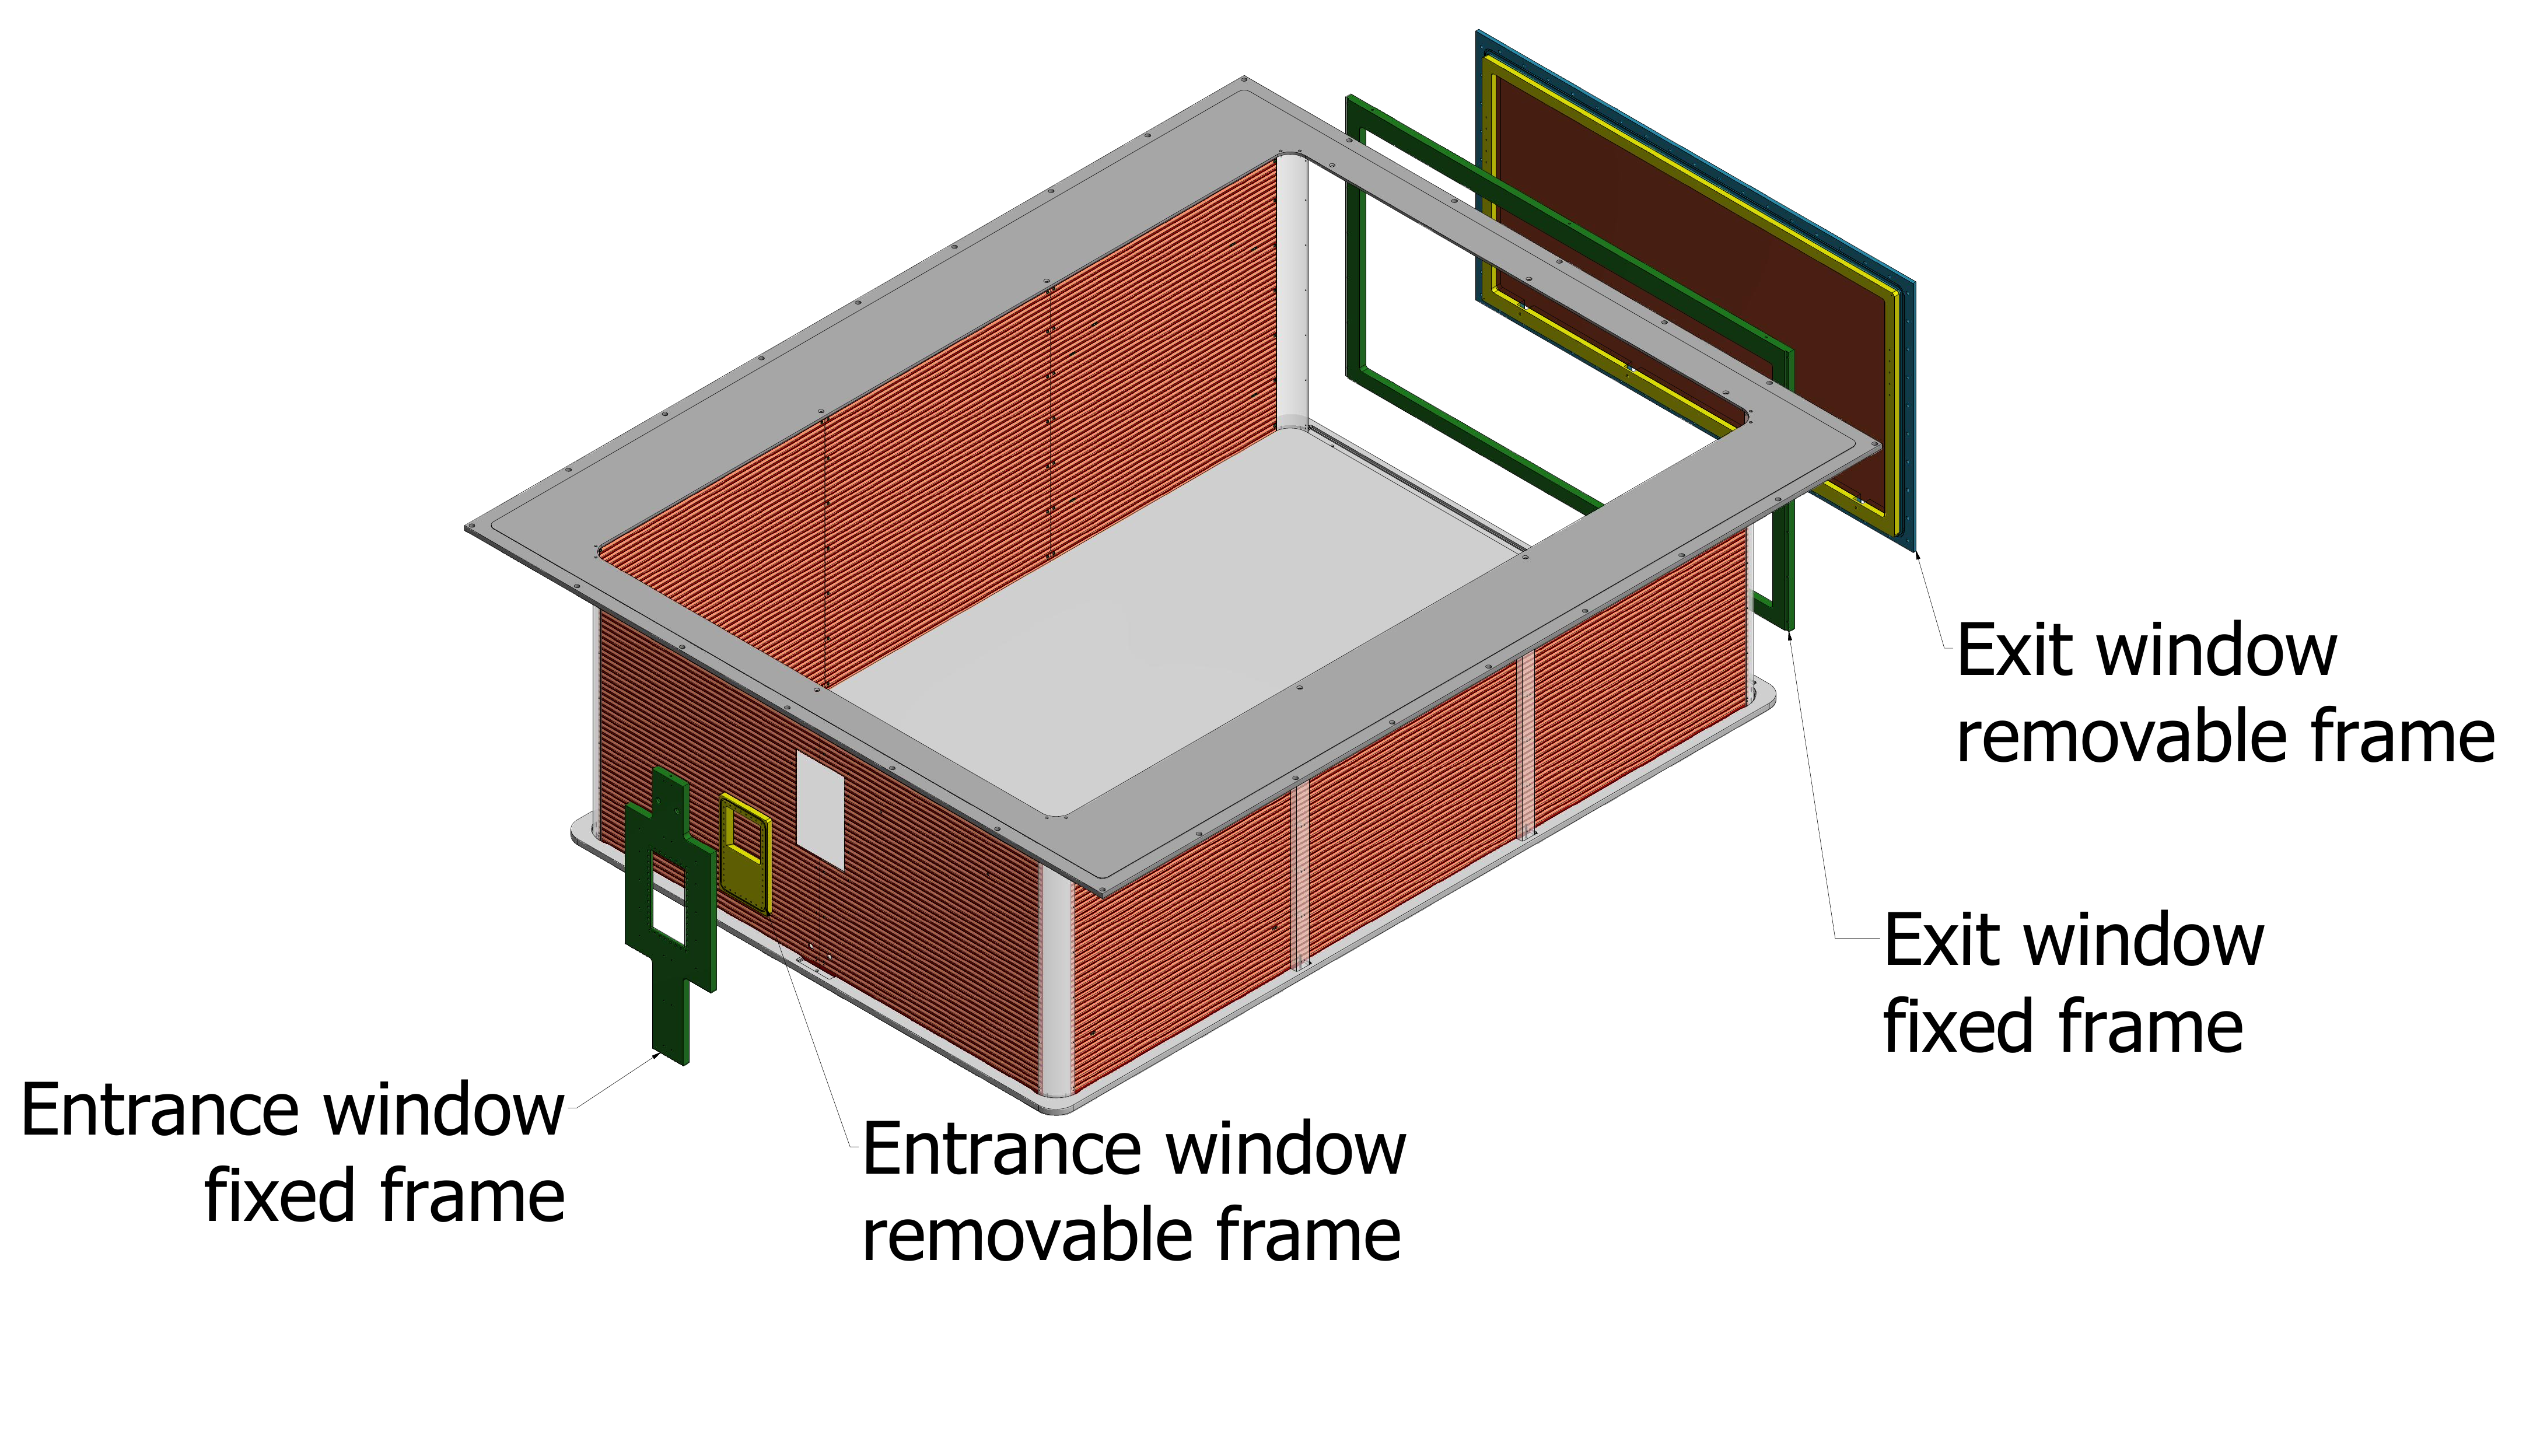
\includegraphics[width=\textwidth]{fc_overview.png}
\label{fig:fc_overview}
\caption{FC overview}
\end{figure}


\begin{figure}[!htb]
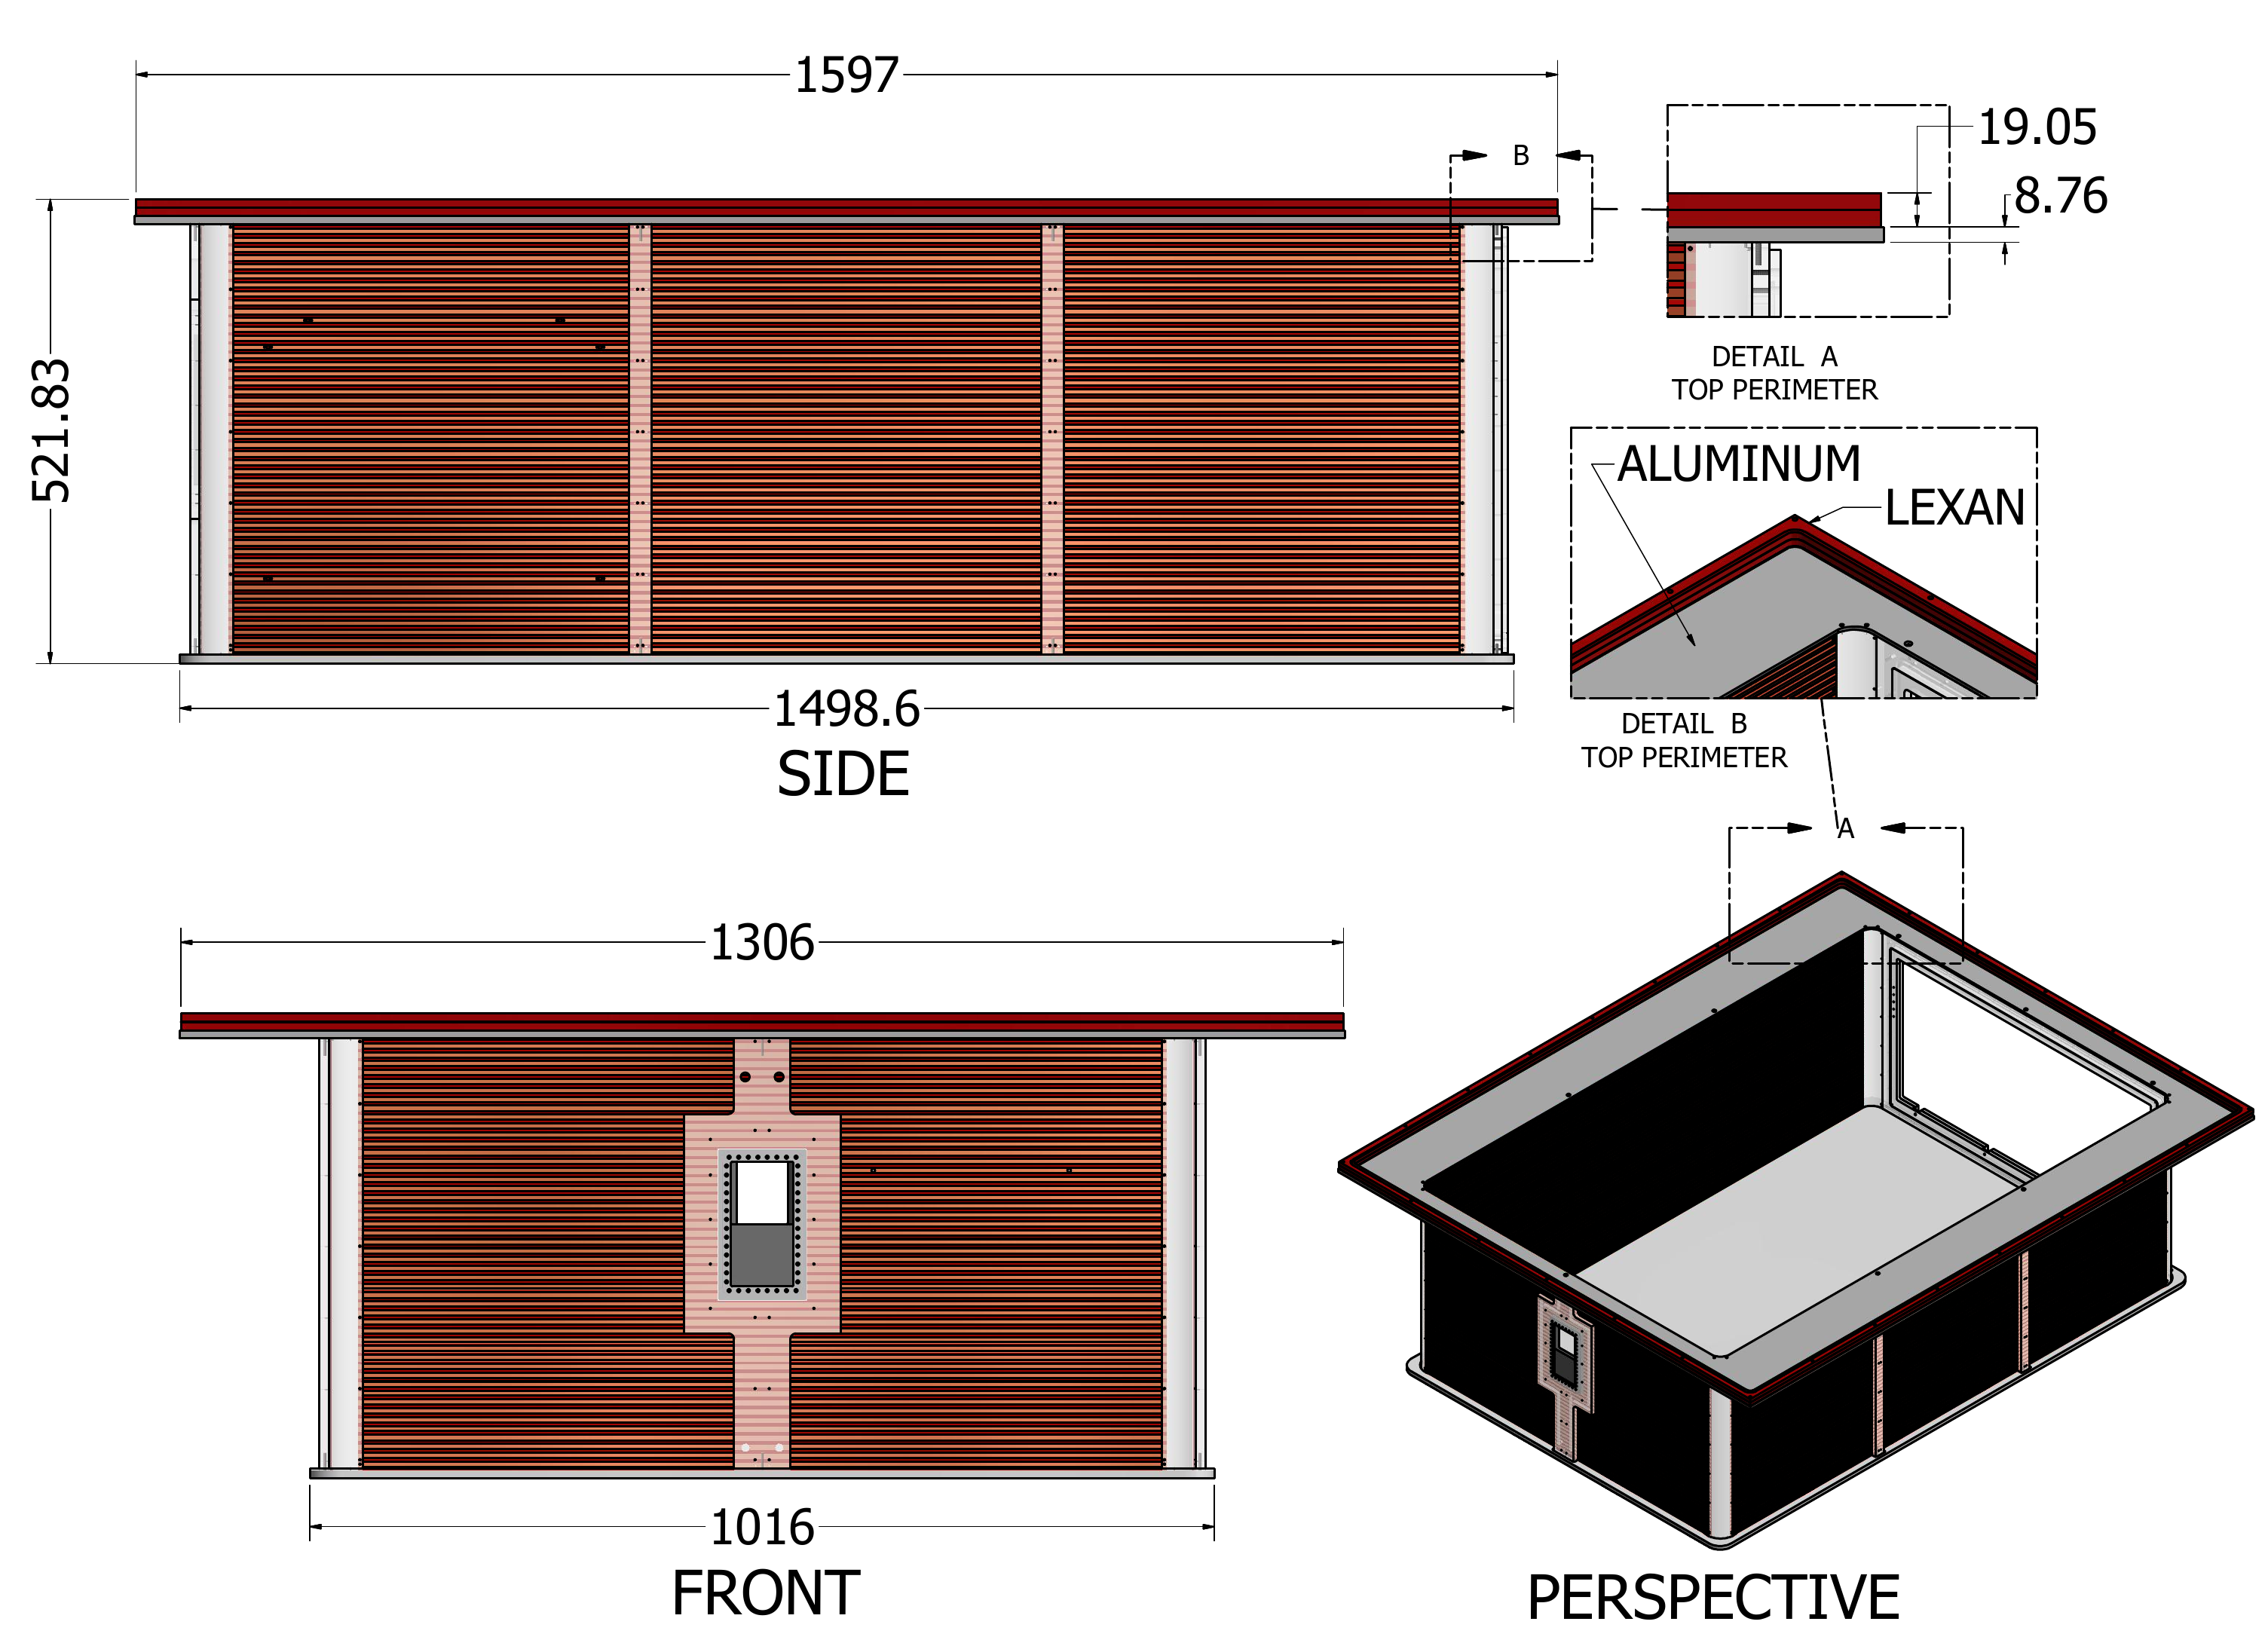
\includegraphics[width=\textwidth]{fc_overview2.png}
\label{fig:fc_overview2}
\caption{FC overview 2}
\end{figure}

The field cage was constructed from several panels of printed circuit boards (PCBs). The front of the field cage was made of two PCBs and each side was constructed of three PCBs supported by Lexan pieces. The epoxy in the common PCB substrate FR4 contains bromine which is not suitable for the long term operation of a TPC, as the bromine will eventually cause gain reduction of the wires \cite{tpcAging}. The halogen free material used was Cryogenic-G10.  The field cage is an isolated volume from the enclosure of the TPC for the option to run explosive gases such hydrogen in the field cage, where the enclosure can be filled with an insulating gas. While the risk of a high voltage spark was minimized using the voltage step down, the risk of sparking when using an explosive gas could be further minimized by isolating the detector volume from the enclosure volume thereby allowing you to run an insulating gas between the field cage while running the explosive gas inside the detector volume only. Instead of a downstream wall, a large thin exit window was constructed which consisted of a lexan frame bonded to a \SI{10}{\micro\metre} Kapton window with evaporated aluminum strips. The PCB boards were epoxied into the cathode which was constructed of an aluminum honeycomb laminate where two sheets of aluminum were bonded to a core of aluminum honeycomb structure providing a lightweight yet rigid structure. On the other end the boards were epoxied into an aluminum top perimeter which also served as the last ring in the TPC. Together with the cathode bottom, the field cage proved to be a rigid lightweight structure. A lexan ring containing o-rings was placed in-between the top perimeter piece and the top plate of the TPC. Screws with nylon washers, and collars, were used to mount the top perimeter, and the field cage, to the top plate. The top plate could be removed and rotated with the field cage on without damaging any internal components. 

\begin{figure}[!htb]
\centering
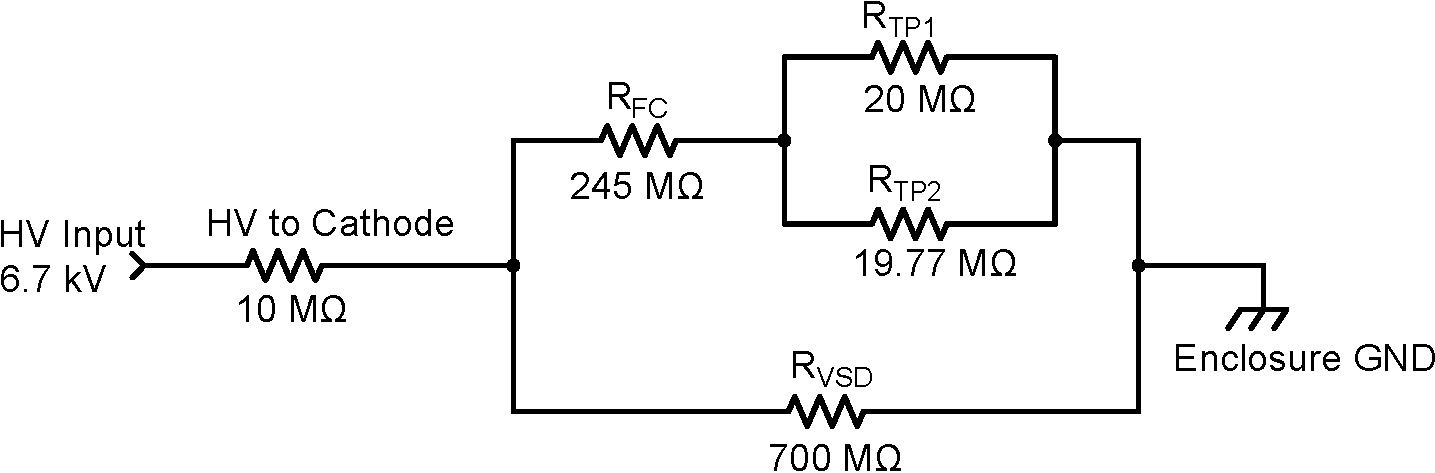
\includegraphics[width=\textwidth]{TPC_schematic.pdf}
\caption{Schematic of the TPC system}
\label{fig:TPC_schematic}
\end{figure}

The cathode is connected to the HV supply through a \SI{10}{\mega\ohm} resistor and has an effective capacitance to ground of \SI{4}{\nano\farad}, $C_{VSD}$. The cathode voltage $V_{cath}$ can be calculated from the schematic of the TPC system in Fig.~\ref{fig:TPC_schematic}, as
\begin{equation}
V_{cath} = \frac{V_{HV}}{ 1 + \frac{10}{ \left( (245 + R_p)^{-1} + 700^{-1} \right)^{-1} } },
\end{equation}
where 
\begin{equation}
R_p = \left( R_{TP1}^{-1} + R_{TP2}^{-1} \right)^{-1},
 \label{eq:Reff}
\end{equation} 

is the effective resistance of the last resistor, and $V_{HV}$ is the high voltage supply; all resistor values are given in \si{\mega\ohm}.


\begin{figure}[!htb]
\centering
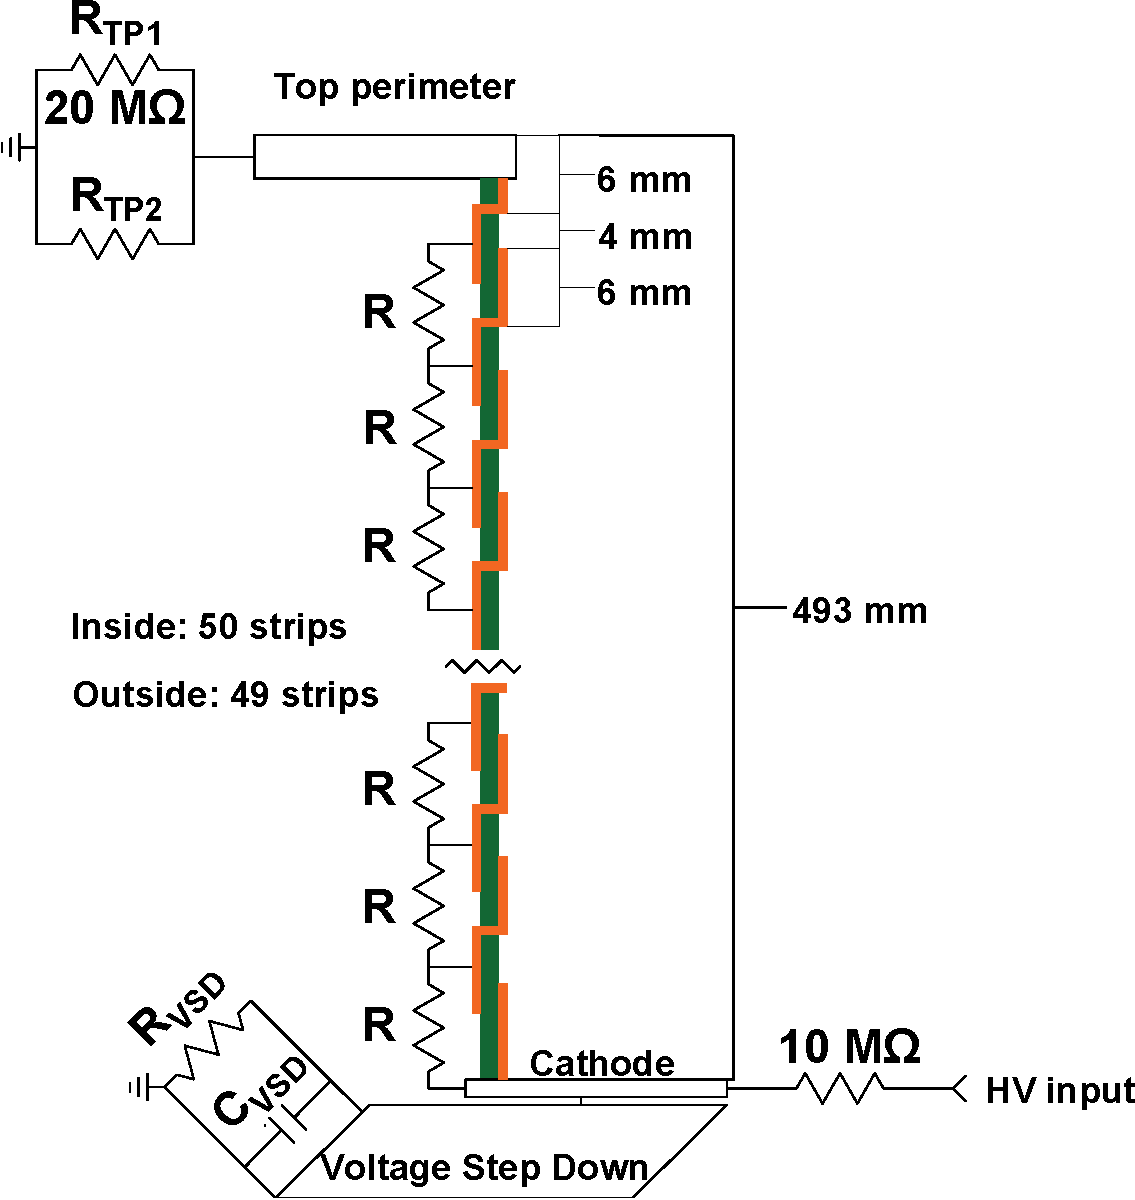
\includegraphics[scale=.6]{FC_schematic.pdf}
\caption{Schematic of the electric connections relevant to the Field Cage system. The strip thickness is exaggerated in the figure to show the detail}
\label{fig:FC_schematic}
\end{figure}

Figure~\ref{fig:FC_schematic} shows a cartoon schematic of the field cage walls. The field cage contains 50 inside copper strips and 49 outside copper strips. The strips on each board was connected to the adjacent strip on the next board; front, back, and side boards were connected by G10 corner pieces with conducting paint strips, creating rings around the whole field cage. The first inside strip is connected to the cathode, which is itself connected by an effective \SI{5}{\mega\ohm} resistor ($R$) to the first outside strip. The first outside strip is connected trough a via to the second inside strip, which continues on in this repeating fashion. The resistor chain creates a voltage divider in which each strip is separated by a constant difference voltage at a fixed distance, setting up a constant electric field. The last strip of the field cage is composed of a small inner strip  (\SI{1.5}{\milli\metre}) on the PCB board and the aluminum top perimeter piece (\SI{4.5}{\milli\metre}) giving an  effective thickness of \SI{6}{\milli\metre}, the same as the other strip widths. The top perimeter is connected to electrical ground through a \SI{20}{\mega\ohm} resistor ($R_{TP1}$) with the option to place an additional resistor ($R_{TP2}$) in parallel to tune the voltage of the top perimeter, as seen in Fig.~\ref{fig:FC_schematic}. 

The voltage on each strip, $V_n$, can be expressed as, 
\begin{equation}
V_n = V_{cath} \frac{R_p + (50 - n)R}{49\cdot R + R_p}
\label{eq:FCstrip}
\end{equation}

where $n = 1$ represents the index of the first inside strip, and $n= 50$ represents the index of the last inside strip, which is the same as the top perimeter voltage.

%Talk about the uniforminty of the field cage maybe
%how far the wall was from the pad plane on the sides talk about the front


\subsection{Voltage Step Down}
The gap between the field cage's cathode and the ground of the enclosure is quite small. To prevent electric breakdown in the gas between this gap a series of concentric copper rings safely stepped down the voltage to ground; where each ring was separated by a resistor. There were 8 concentric rings with a \SI{10}{\mega\ohm} resistors in between, creating a resistor chain which steps down the voltage each ring by approximately \SI{1000}{\volt} each time. The first ring is the same voltage as the cathode and the last ring is connected to ground. All together the total resistance of the resistor chain is \SI{700}{\mega\ohm}.


\subsection{Wire Planes}
%Add figure of gating grid transparency closed and open configuration 

There are three wire planes that are mounted underneath the pad-plane. The wire plane closest to the pad-plane (\SI{4}{\milli\metre}) are the anode wires. The next plane (\SI{12}{\milli\metre}) is the ground plane or frisch grid, and the last plane (\SI{14}{\milli\metre}) is the gating grid. The gating grid is the first plane that electrons meet as they drift upward from the field cage volume towards the anode plane. The gating grid is operated as a gate either allowing electrons and ions through, or blocking them entirely. The ground plane functions to shield the inside volume of the TPC from the high electric field surrounding the anode wires where the avalanche process of the electron takes place. The ground plane is the least interesting plane and is shorted to the enclosure ground by a BNC terminator on the outside of the TPC. If we would like to calibrate the electronics of the TPC we typically inject a pulser into one end of the ground plane and terminate the other end with a \SI{50}{\ohm} termination.  


 \begin{table*}[!htb]
 \centering
\ra{1.3}
\begin{tabular}{@{}rrrrrrr@{}}\toprule 
\multicolumn{2}{c}{GET electronics settings}\\
\midrule
 Plane & Material & Diameter \si{\micro\metre} & Pitch \si{\milli\metre} & Distance to pad-plane & Tension \si{\newton} & Voltage \si{\volt}\\ [0.5ex] 
 Anode  & Au-plated W   &  20  &  4  &  4   &  0.5  &  1460  \\
 Ground & BeCu          &  75  &  1  &  8   &  1.2  &  0     \\ 
 Gating & BeCu          &  75  &  1  &  14   &  1.2 &  -110$\pm$ 70\\ 
 \bottomrule
\end{tabular}
\caption{Wire plane properties}
\label{tb:wireplane}
\end{table*}

In the open configuration the gating grid is transparent to electrons coming from the field cage volume and also allows for ions to move from the avalanche region into the TPC volume. Typically the gating grid is held in the closed configuration only opening when the data acquisition trigger criteria is met. This is to block the electrons which come from the un-reacted beam, which happens frequently, which if allowed to go to the anode wires, would quickly build up enormous amounts of positive ions and flood the volume of the field cage with space charge. We close the gating grid after reading out approximately one TPC volume -- about \SI{10}{\micro\second}  -- to also prevent the back-flow of ions from the avalanche region from that event. Since ions move with a velocity much slower than that of elections, the ions only move several \si{\micro\metre} in the time the gate is open; this allows for electrons to pass through while preventing the back-flow of ions into the FC volume. 

Figure~\ref{fig:gg_onoff} shows a Garfield simulation of the gating grid in both the on and off configurations. In the on configuration, all the wires share the same average voltage, $V_{g.g.}$, which is optimized for the case of 100\% electron transparency. In the off configuration, the reference voltage $V_{g.g.}$ remains the same, but alternating wires get an offset voltage of $\pm \Delta V$, so that the electric field produced by the voltage difference $2\Delta V$ between wires is great enough to block incoming electrons. Opening the grid from this closed bi-polar mode is simply done by removing the offset voltage and allowing the two wires to short which equilibrates their charges, which is the state of the reference voltage. 

\begin{figure}[!htb]
    \centering
    \begin{subfigure}[t]{0.49\textwidth}
        \centering
        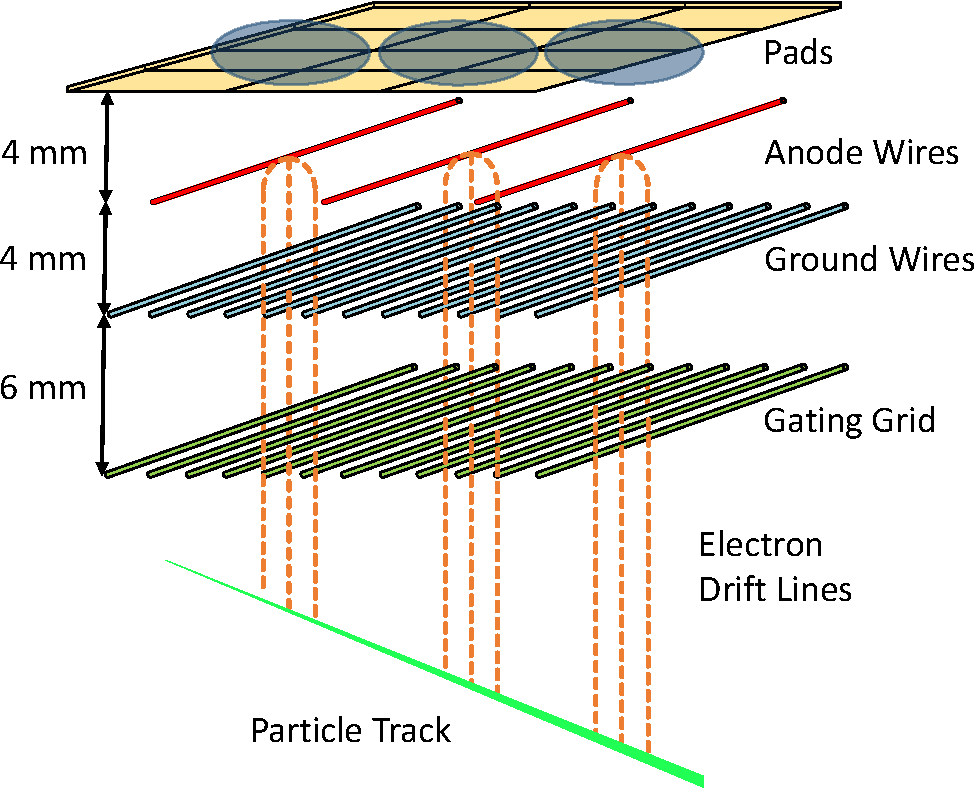
\includegraphics[width=\linewidth]{wires_open.pdf} 
        \caption{Wires open} \label{fig:wires_open}
    \end{subfigure}
    \hfill
    \begin{subfigure}[t]{0.42\textwidth}
        \centering
        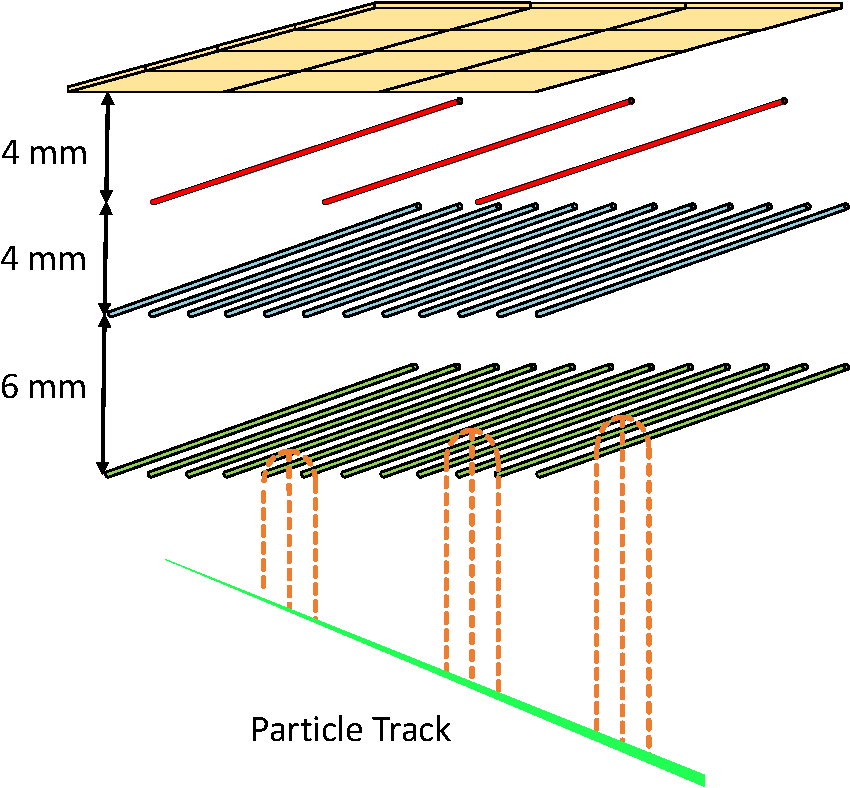
\includegraphics[width=\linewidth]{wires_closed.pdf} 
        \caption{Wires closed.} \label{fig:wires_closed}
    \end{subfigure}
\label{fig:wires}
\end{figure}



\begin{figure}[!htb]
\centering
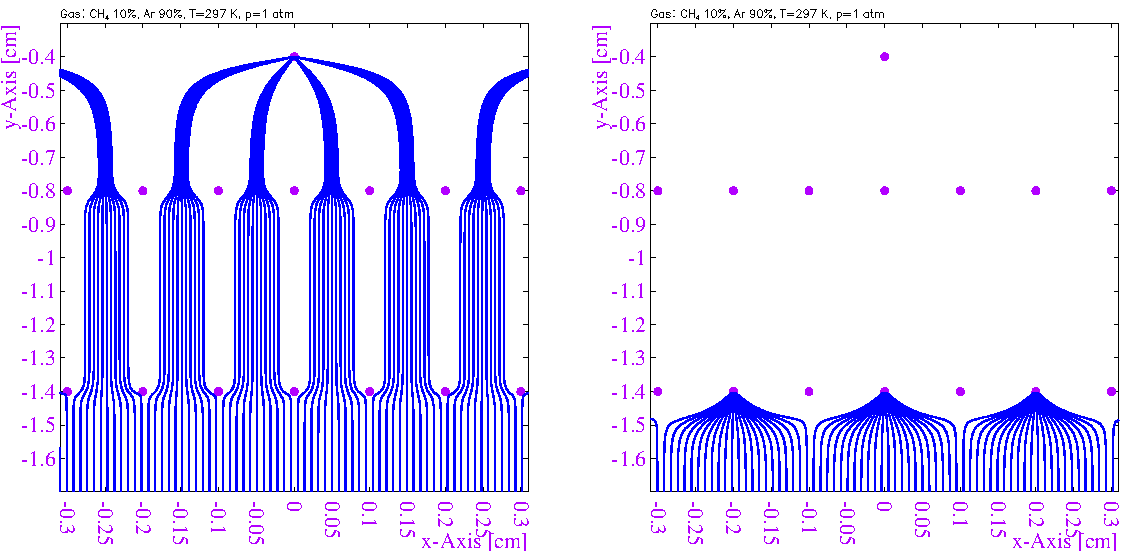
\includegraphics[width=\textwidth]{gg_onoff.pdf}
\caption{On and off configurations of the gating grid.}
\label{fig:gg_onoff}
\end{figure}


Both configurations of the gating grid were measured and simulated. To measure the electron transparency were all wires share the voltage $V_{avg}$, the anode wire was lowered to \SI{500}{\volt} and the beam was allowed to enter the field cage without any target put in. By lowering the voltage of the anode we could measure the large charge of the beam without saturating the electronics. The average charge deposited in the chamber could be measured as a function of $V_{avg}$; changing the top plane resistor appropriately according to Eq.~\ref{eq:TP_resistor}. Several runs were taken ranging from \SIrange{-198}{-40}{\volt}, with and without the magnetic field. Theoretically the most negative value represents 100\% electron transparency and was used as the reference run. The electron transparency, $T$, was defined as $T = \langle dE/dx\rangle/{\langle dE/dx\rangle}_{ref}$, where $\langle dE/dx\rangle_{ref}$ represents the average energy loss of the reference run. Figure~\ref{fig:ggAvgTrans} shows the measured transparency as a function of $V_{avg}$, as compared with the corresponding Garfield simulation. The average gating grid voltage used in the experiment was \SI{-171}{\volt} to ensure we were well within the 100\% transparency region. 

To measure the electron transparency as a function of the difference voltage $\Delta V$, the average voltage was first set to 100\% transparency, $V_{avg}=\SI{-171}{\volt}$, and the difference voltage was added or subtracted from alternating wires. Figure~\ref{fig:ggDeltaVTrans} shows the result of the simulation and experiment with and without the magnetic field. By introducing the magnetic field the required voltage to close the grid increases. In the experiment we selected the value of $\Delta V = \SI{65}{\volt}$ to ensure we were well within the region of 0\% transparency.  

\begin{figure}[!htb]
    \centering
    \begin{subfigure}[t]{0.49\textwidth}
        \centering
        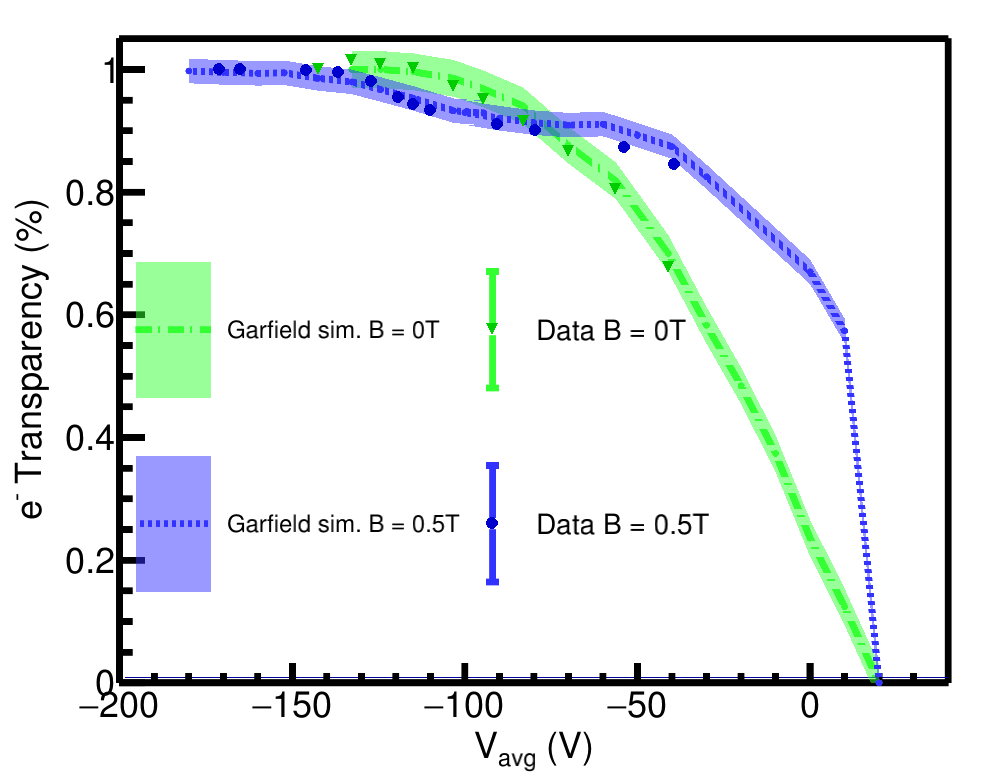
\includegraphics[width=\linewidth]{averageTransparency.png} 
        \caption{Electron transparency for the conditions of all wires are the same voltage.} \label{fig:ggAvgTrans}
    \end{subfigure}
    \hfill
    \begin{subfigure}[t]{0.49\textwidth}
        \centering
        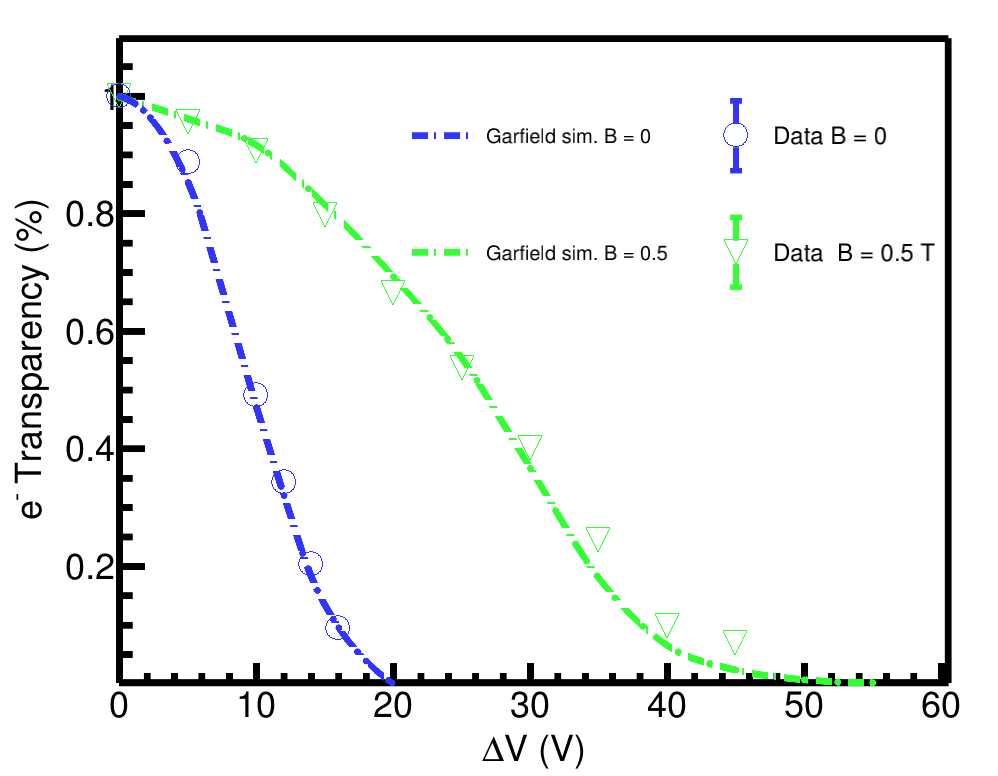
\includegraphics[width=\linewidth]{transparencyDeltaV.png} 
        \caption{Electrons transparency for the mode where adjacent wires have a voltage difference of $2 \Delta V$.} \label{fig:ggDeltaVTrans}
    \end{subfigure}
\label{fig:ggTrans}
\end{figure}



The anode wires are made of very thin Gold plated Tungsten wires, about \SI{20}{\micro\metre} in diameter. They are biased to high voltages around \SI{e3}{\volt} which creates a very high electric field very close to the anode wire. As the eletron drifts towards the anode wire, it gains kinetic energy knocking out more electron-ion pairs in the gas until it terminates on the anode wire or the pad plane. The amount of electrons produced depends on the anode wire voltage and the gas properties. The absolute gas gain was not experimentally measured but was calculated in a Garfield simulation. During the experiment the anode wires were biased to two different voltages. We will refer to the voltage \SI{1460}{\volt} as the ``high voltage" and \SI{1214}{\volt} as the ``low voltage". Only two sections were biased with the lower voltage setting due to concerns of a high current issue. Figure~\ref{fig:anodegain} shows the expected number of electrons distributions for electrons produced in a avalanche process of an electron creating a single avalanche. The distribution follows the expected Polya distribution and the MC data in the simulation was fitted with a Polya function \cite{blumrol}, described as,

\begin{equation}
P(x) = A_0^{-1}\cdot \frac{A_1^{A_1}}{\Gamma(A_1)} \left(\frac{x}{A_0}\right)^{A_1-1}e^{\frac{-A_1x}{A_0}}.
\end{equation}

For the voltage of \SI{1460}{\volt} the parameters of the fit are $A_0=903.9$ and $A_1=1.50$ and for the voltage of \SI{1214}{\volt} the parameters are $A_0=150.0$ and $A_1=1.47$. 



\begin{figure}[!htb]
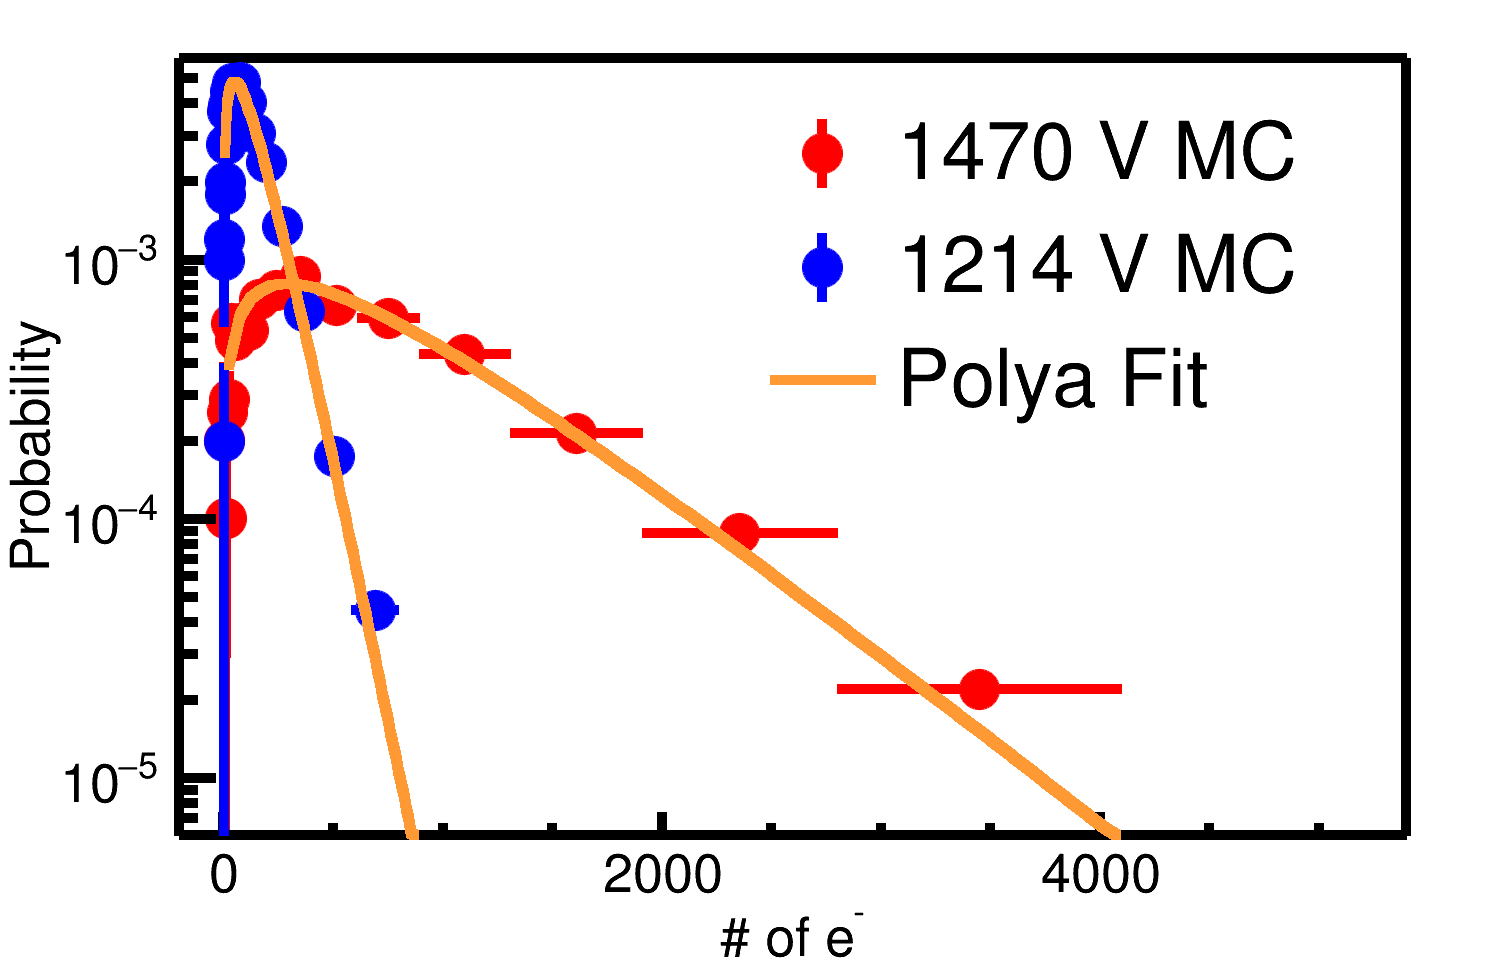
\includegraphics[width=\textwidth]{gain.png}
\caption{Number of electrons produced in a single avalanche on an anode wire. Two different voltages were simulated using Garfield++ at 1470 $V$ and 1214 $V$. The expected Polya distribution fit is also given in yellow.}
\label{fig:anodegain}
\end{figure}


The wire plane and the cathode define the different electric field regions. The main drift region is defined by the space between the gating grid and cathode voltages (Region 1), with a small drift region being defined by the space between the ground grid and the gating grid (Region 2); the avalanche region is defined as between the ground grid and the anode grid. The voltage of the gating grid is set to the point that allows for 100\% transparency for electrons. It is possible that the electric field in Region 1 and Region 2 can be matched but not required. The voltage of the top perimeter is set by adjusting the value of the last resistor ($R_{TP2}$) to ensure the electric field is constant through Region 1. We can imagine Region 1 is split into two virtual volumes, one defined between the cathode and the top perimeter, and one defined between the top perimeter and the gating grid. The magnitude of the electric field in the region between the top perimeter and the cathode, $E_1$, is defined as,

\begin{equation}
E_1 = \frac{V_{g.g.} - V_{tp}}{ y_{g.g.} - y_{tp} },
\end{equation}
where  $V_{g.g.}$, $V_{tp}$ , $y_{g.g.}$, and $y_{tp}$ are the voltage and vertical y-position of the gating grid and top perimeter respectively. The magnitude of the electric field in the region between the top perimeter and the cathode, $E_2$, is defined as,

\begin{equation}
E_2 = \frac{V_{tp} - V_{cath}}{ y_{tp} - y_{cath} },
\end{equation}
where  $V_{tp}$, $V_{cath}$ , $y_{tp}$, and $y_{cath}$ are the voltage and vertical y-position of the top perimeter and cathode respectively. The condition for a smooth electric field across the volume is given by $E_1 = E_2$. Substituting Eq.~\ref{eq:FCstrip} for $V_{tp}$ ($n=50$), we can solve for the effective resistance of the top perimeter $R_p$ as, 

\begin{equation}
R_p = 49 \cdot R  \left(\frac{ y_{g.g.} - y_{cath} }{ y_{TP} - y_{cath} \frac{V_{cath} - V_{gg}}{V_{cath}} }- 1 \right),
\label{eq:TP_resistor}
\end{equation}

where the relevant vertical dimensions are $y_{g.g.} - y_{cath} = \SI{497.3}{\milli\metre}$ and $y_{tp} - y_{cath} = \SI{490}{\milli\metre}$. The value of $R_{TP2}$ can be calculated from Eq.~\ref{eq:Reff} and Eq.~\ref{eq:TP_resistor}.


\subsection{Pad Plane}
The pad-plane is a multi-layer circuit board which is segmented into \SI{11.5}{\milli\metre} x \SI{7.5}{\milli\metre} charge sensitive pads; arranged in an array of 108 x 112 pads in the x and z-directions respectively making 12096 pads in total. There is an insulating gap of \SI{0.5}{\milli\metre} on each side separating the pads. The effective area covered by the pads is \SI{1344}{\milli\metre} x \SI{864}{\milli\metre}. There is a via and trace coming from each pad to the opposite side of the pad plane and is arranged in a surface pads which may be readout by a surface mount SAMTEC connector. Figure~\ref{fig:padplane} shows the pad plane boards being glued to the top plate and the holes which allow for the readout of pads. The pads were gold plated for excellent electric conduction properties. 

\begin{figure}[!htb]
\centering
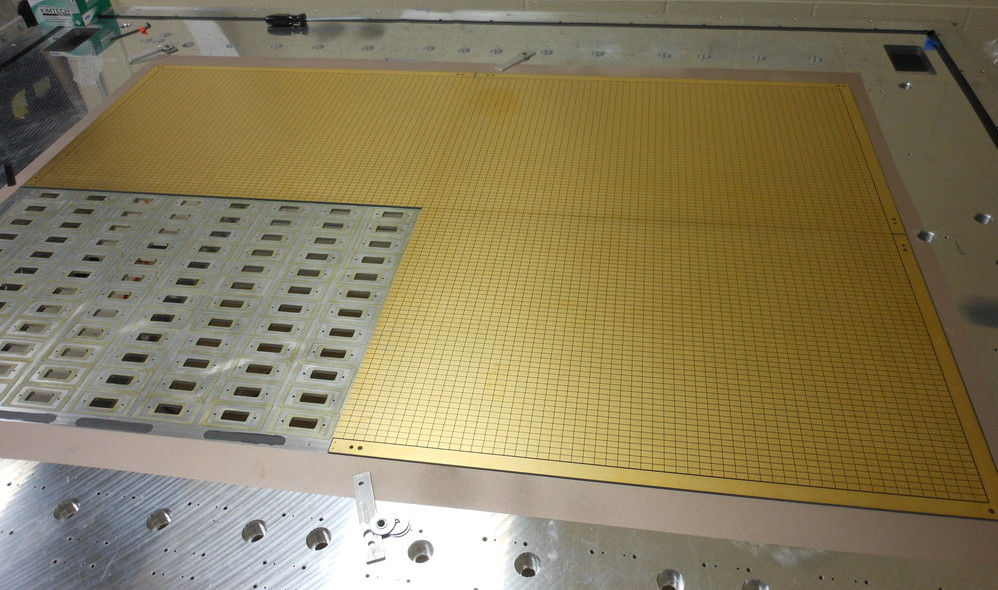
\includegraphics[width=\textwidth]{3boards_ps.jpg}
\caption{Figure of the pad plane boards being glued to the top plate. }
\label{fig:padplane}
\end{figure}


\subsection{Electronics}

Signals in the S$\pi$RIT TPC are amplified and digitized by the recently developed Generic Electronics for TPCs (GET) \cite{get}.  Short cables transmit the signals from the pads to through a circuit protection board called ZAP, to the inputs of the AGET chips mounted to the AsAd board as seen in Fig.~\ref{fig:getzap}. Each AGET chip services 64 pads (63 pads are connected in our case), contains a pre-amplifier, and a Switched Capacitor Array (SCA), with a maximum of 512 time buckets with an adjustable sampling frequency of 1 to 100 MHz. Four AGET chips are mounted on one AsAd (ASIC and ADC) motherboard. The gain of each AGET can be configured as 0.12, 0.24, 1.0, or 10 pC over the whole dynamic range, and the ADCs on each AsAd board provides 12 bit resolution. The peaking times of the shaping amplifiers can be set to 69, 117, 232, 501, 720, or 1014 ns. In this experiment, the gain was set to the highest setting, 0.12 pC, the peaking time 117 ns, and the sampling frequency 25 MHz (resulting in 40 ns time buckets). 

\begin{table*}[!htb]
\centering
\ra{1.3}
\begin{tabular}{@{}rr@{}}\toprule 
\multicolumn{2}{c}{GET electronics settings}\\
\midrule
ADC bit range       & 14 bits \\
Sampling frequency  & 1-100 MHz \\
Dynamic range       & .12, .24, 1.0, 10pC \\
Peaking time        & 69,117,232,501,720,1014 ns \\
Time bucket range   & 512\\
\bottomrule
\end{tabular}
\caption{Summary of range of GET electronics settings. }
\label{tb:getoverview}
\end{table*}

\begin{figure}[!htb]
\centering
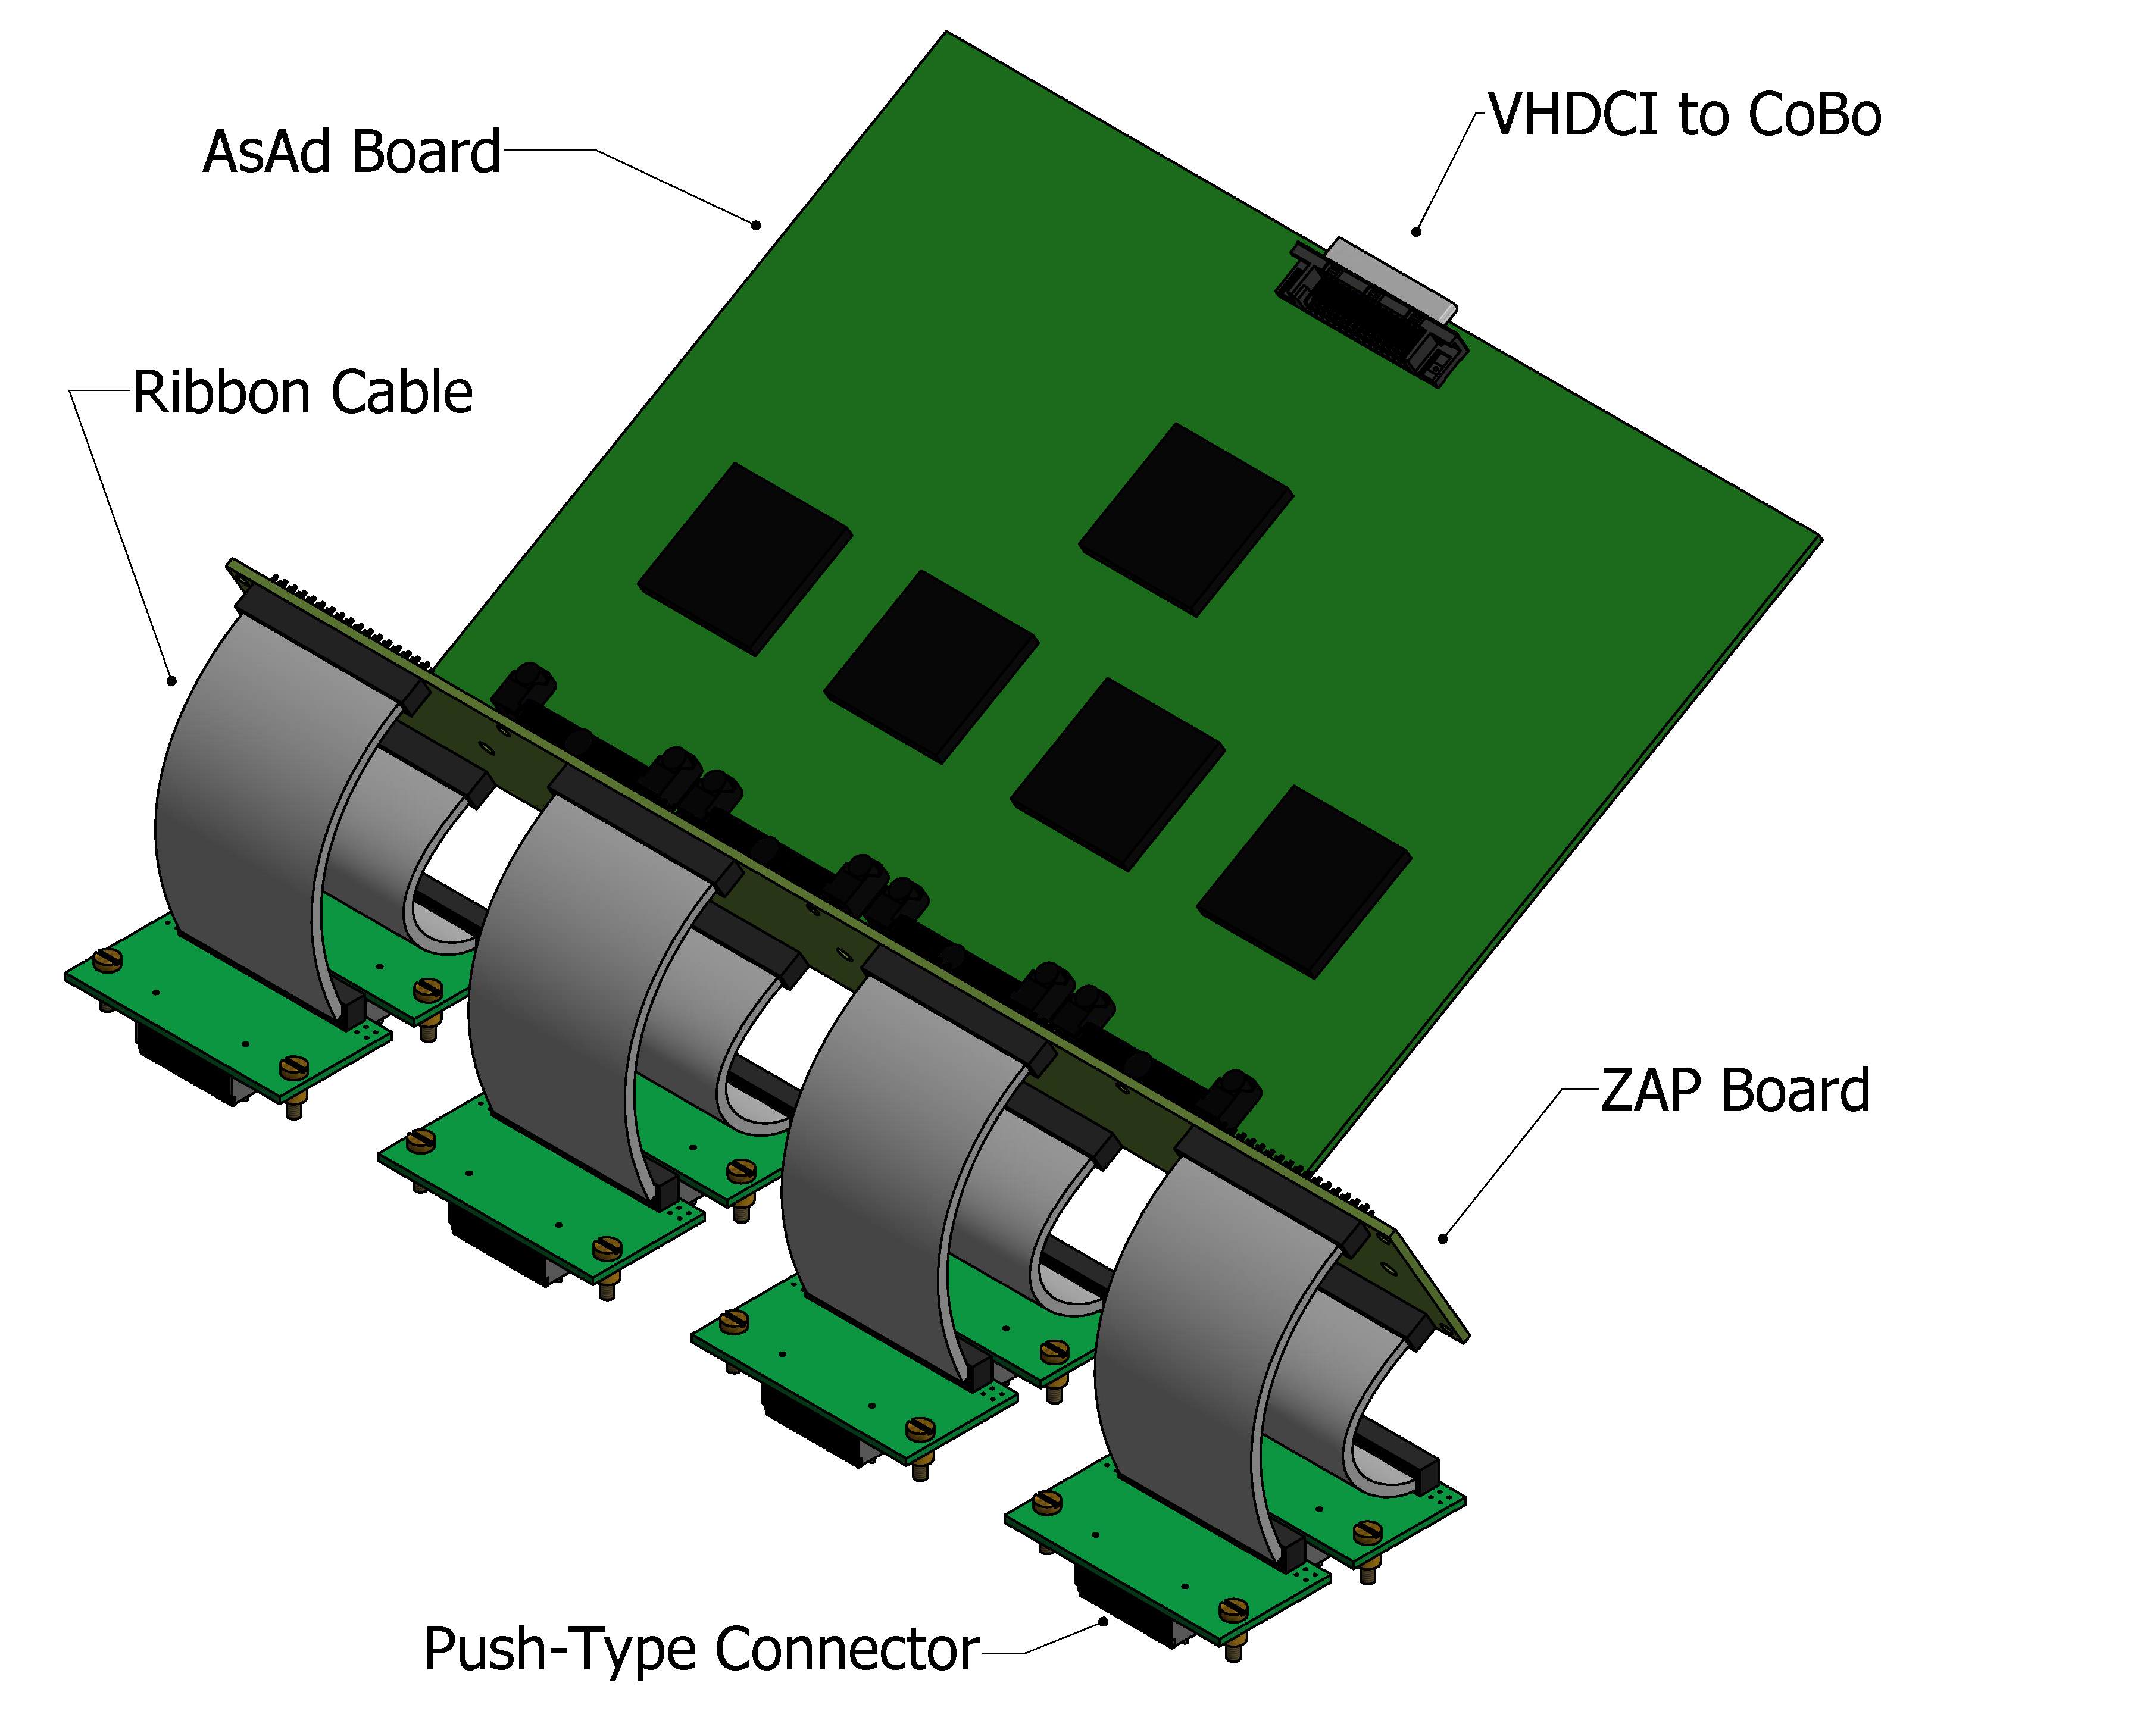
\includegraphics[width=.5\textwidth]{GET_and_ZAP.pdf}
\caption{•}
\label{fig:getzap}
\end{figure}



\begin{figure}[!htb]
\centering
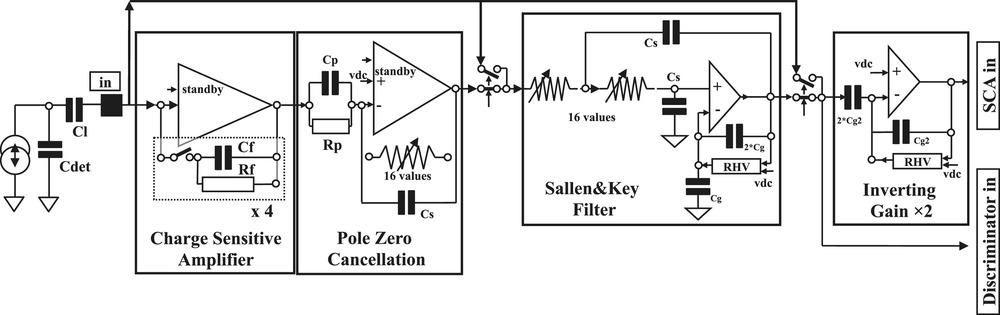
\includegraphics[width=\textwidth]{AGETfncn.jpg}
\caption{Schematic of the internals of the AGET chip from \cite{get2}}
\label{fig:aget}
\end{figure}


\begin{figure}[!htb]
\centering
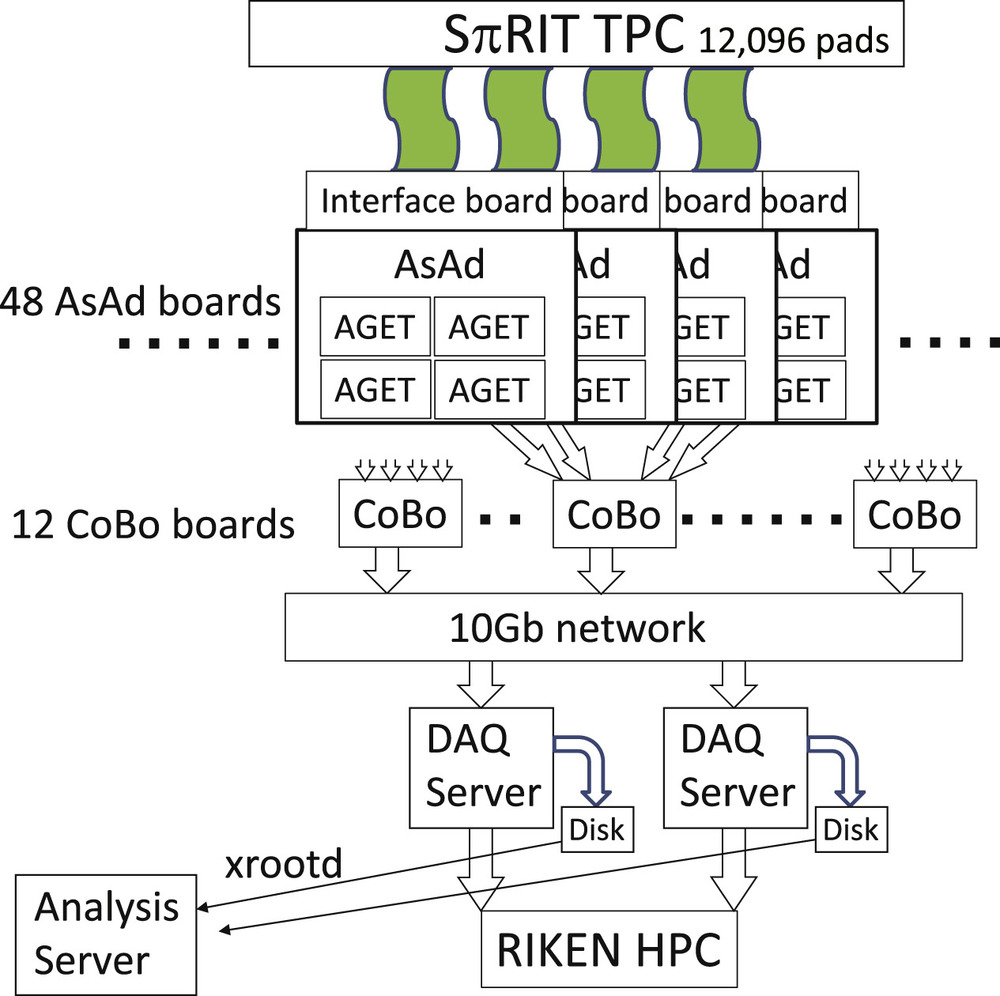
\includegraphics[width=.5\textwidth]{GETlayout.jpg}
\caption{Readout structure of the AsAd boards and CoBo board structures. Also the relevant components of the DAQ system.}
\label{fig:coboDAQ}
\end{figure}

After each AsAd board has digitized the data it is sent to the Concentration Boards (CoBo). Each CoBo board can concentrate the data from 4 AsAd boards. The Multiplicity, Trigger, and Time module (MuTanT) \cite{get} provides the common trigger signal for all CoBo boards.  Each board sends the data to the DAQ server which writes to disk the data from each board, which was handled by two separete DAQ servers; saving to one common analysis server. The data could then be analyzed using the RIKEN High Performace Computing cluster or moved to the NSCL or MSU cluster for analysis. The Aget 2.0, asad 2.1, and cobo 1.0 firmware versions were used. 

\section{Energy loss in material}
The average energy loss in a material can be described by the Bethe-Bloch equation,
\begin{equation}\label{eq:bb}
\frac{dE}{dx} = \frac{4\pi NZ^2e^4}{mc^2\beta^2} (ln \frac{2mc^2\beta^2\gamma^2}{I} - \beta^2).
\end{equation}
Where $N$ is the number density of electrons in the medium, $e$ the elementary charge, $mc^2$ is the rest mass of the electron, $Z$ is the charge of the traversing particle, $I$ is the mean excitation energy of the medium, and $\beta$ is the velocity of the particle. There is a large variation in energy loss around this mean value, with a long high energy loss tail. 

The statistical variation of energy loss in a material was described by Landau \cite{landau} and later better described by Shulek \cite{shulek} and Bichsel \cite{bichsel1}. In both approximations it is described by a most probable energy loss value with a long, high-energy loss tail. Because of this long tail, for a finite set of energy loss measurements along a given track, the fluctuation of the mean value energy loss is a very unreliable observable. The most probable energy loss is the most desirable observable either through fitting of the observed distribution or through the truncated mean method. The solid curve in Fig.~\ref{fig:straggling} shows the energy loss distribution in Ar gas for a proton with momentum \SI{3.4}{\giga\eVperc}. The dashed line is the distribution under the Landau assumptions. The mean energy loss $\langle\Delta\rangle$ is significantly shifted from the most probable value $\Delta_p$, due to the long high energy tail. 

\begin{figure}
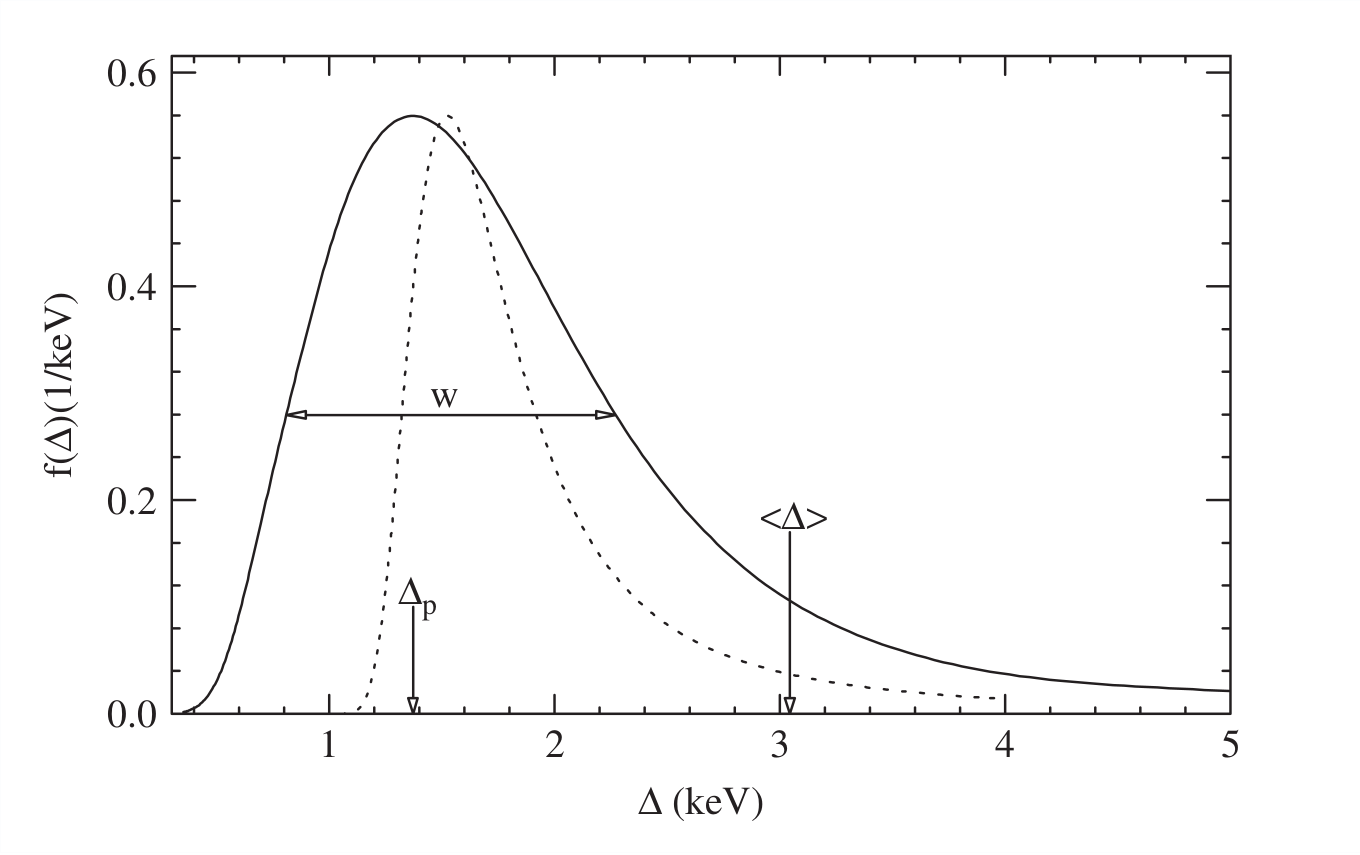
\includegraphics[width=\textwidth]{bichsel.png}
\caption{Energy loss of a $\beta\gamma$ = 3.6 particle in Ar gas taken from \cite{bichsel}}
\label{fig:straggling}
\end{figure}

The truncated mean is the average mean value calculated after throwing away the top fraction of the highest energy loss entries. This approximates the most probable value without performing a fit to a known distribution. To calculate the truncated mean $C$, the $n$ energy loss values in a given track $\Delta_i/x$ are sorted from smallest to largest, and the mean value of a reduced set of points $n_t = f_r n$ is calculated as,

\begin{equation}
C = \frac{1}{n} \sum\limits_{i}^{n_t} \Delta_i/x,
\end{equation}

where $f_r$ is the cut off fraction; in this thesis, a value of 0.7 was used. 




%Suppose $E$ represents the set of $N$ energy loss points measured, sorted from lowest to highest energy loss. The $j^{th}$ index marks the position where  $i > j$ entries represent the highest value of energy loss measurements, where their fraction of the total set is expressed as, $f_c = \sum_{i>j} E_i/ \sum_i E_i$. The truncated mean is expressed as the mean value of the remaining energy loss measurements, throwing away the top $f_c$ fraction, expressed as,

%\begin{equation}
%\langledE/dx\rangle_t = \frac{\sum_{i < j} E_i}{N}
%\label{eq:truncatedM}
%\end{equation}

 %A full description of the energy loss distribution can be described in CITE HERE.


\subsection{Gas Properties}
The gas contained by the field cage was a mixture of 90\% Ar and 10\% Methane ($\mathrm{CH_4}$) by volume (P10 gas), and operated just under atmospheric pressure 1 atm. The  gas was continually flowed through the field cage and exited into the enclosure volume, finally passing through a bubbler to atmosphere. The gas purity was monitored with an oxygen and water monitor which are the two most concerning contaminants. The water never exceed  ??? ppm  and the oxygen level never exceeded ??? ppm. Figure~\ref{fig:driftvel} shows the drift velocity of P10 gas at 1 atm (\SI{760}{\torr}) as a function of the reduced electric field value given in units of \si{\volt\per\centi\metre\per\torr}. Operating near the peak value of the drift velocity curve minimizes the change in the drift velocity as the effective field slightly changes due to slight variations in the pressure. The electric field in the experiment was \SI{125}{\volt\per\centi\per\metre} at \SI{760}{\torr}, giving a reduced electric field \SI{0.17}{\volt\per\centi\metre\per\torr}.

\begin{figure}[H]
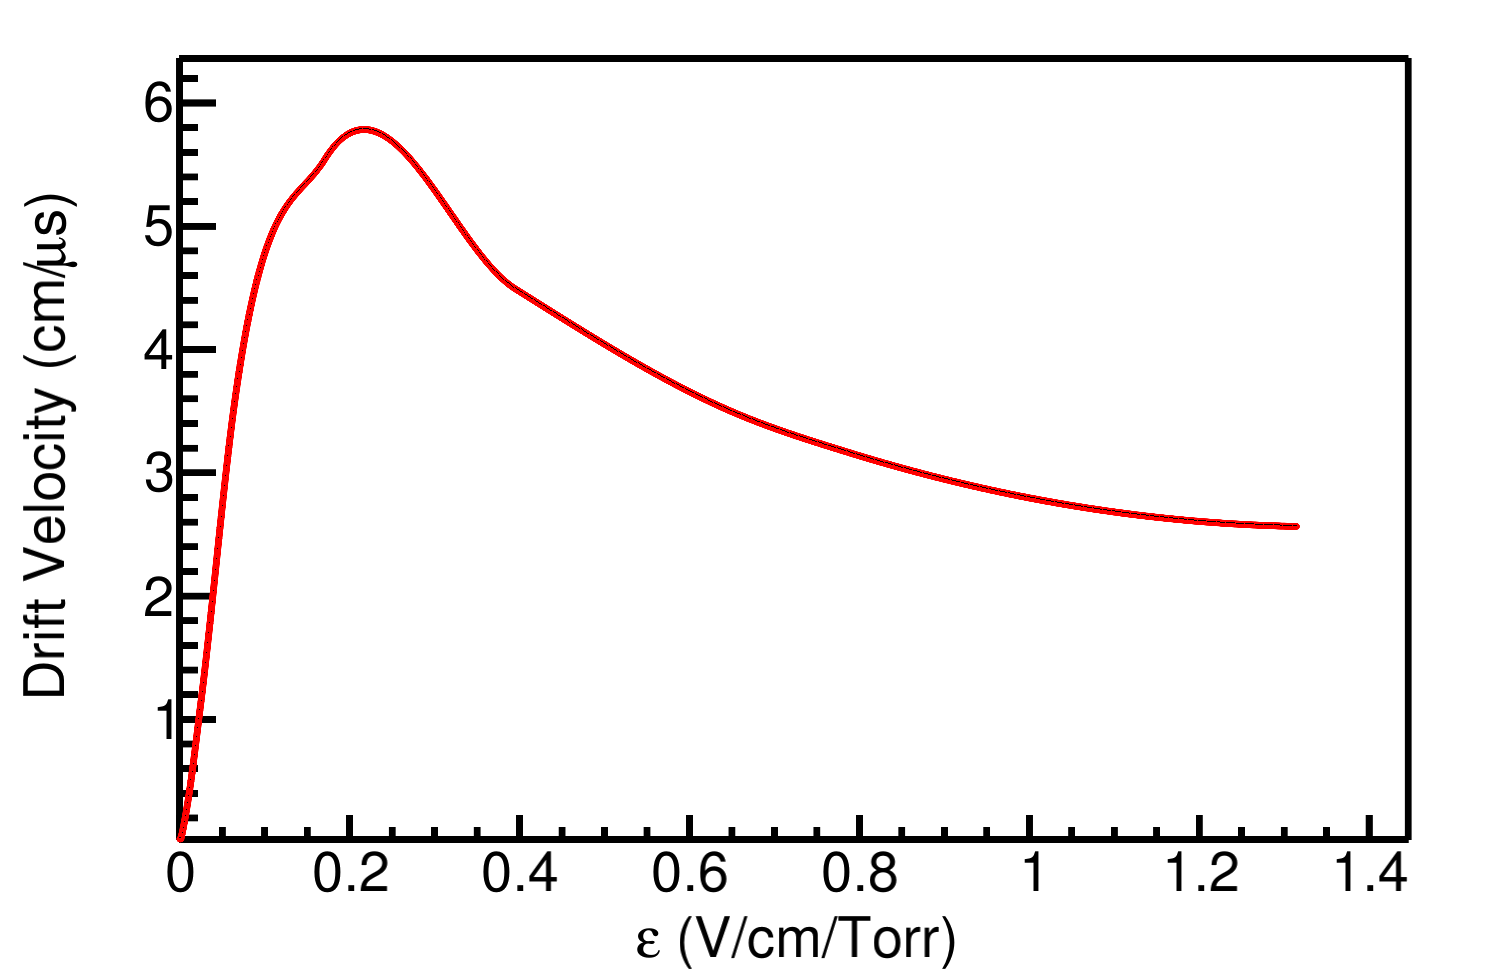
\includegraphics[width=\linewidth]{driftvel.png}
\caption{Drift velocity of electrons in P10 gas.}
\label{fig:driftvel}
\end{figure}

The general formula for the drift velocity, $d\vec{x}/dt$, of an electron in the presence of electric and magnetic fields, $\vec{E}$ and $\vec{B}$, can be expressed in the Langevin equation as,  

\begin{equation}
\frac{d\vec{x}}{dt} = \frac{\mu}{1+(\omega\tau)^2}\Big(\vec{E} + \omega\tau\frac{\vec{E}\times\vec{B}}{|\vec{B}|}+\omega^2\tau^2\frac{\vec{E}\cdot\vec{B}}{|\vec{B}|^2}\vec{B}\Big),
\label{eq:elecdrift}
\end{equation}

where $\mu$ is the signed drift velocity, $\omega$ is the cyclotron frequency, and $\tau$ is the collision parameter for a particular gas \cite{blumrol}.

Several properties of the gas were also simulated in Garfield such as the longitudinal and transverse diffusion, $\sigma_l$ and $\sigma_t$ respectively, and the electron and ion drift velocities, $v_d$ and $v_i$ respectively for the experimental electric field of \SI{125}{\volt\per\centi\metre}; summarized in Table~\ref{tb:gasprop}.


\begin{table}[!htp] % not just 'h!'
\centering % not a center environment
\begin{tabular}{
  @{}
  l
  S[table-format=1.2]
  S[table-format=1.2]
  S[table-format=1.2]
  S[table-format=1.2]
  S[table-format=5.2]
  S[table-format=5.2]
  @{}
}
\toprule
Gas properties &
 {$\sigma_{t}$} &
 {$\sigma_{l}$} &
 {$v_{d}$} &
 {$v_{i}$}  &
 {$G_{h}$} &
 {$G_{l}$} \\
&
  {($\si{\centi\meter}^{-1/2}$)} &
  {($\si{\centi\meter}^{-1/2}$)} &
  {(\si{\centi\meter\per\micro\second})} &
 {(\si{\centi\meter\per\micro\second})} \\

\midrule
\phantom{abc}   &.024   &.034  &5.43  &  \num{2.05e-4} &  903   &150     \\
\bottomrule
\end{tabular}

\caption{}
\label{tb:gasprop}
\end{table}


%Add table for gas diffusion 

\section{Pad Response Function}
\label{sec:prf}
Each electron avalanche produces an two-dimensional image charge on the pad plane, as shown in the cartoon in Fig.~\ref{fig:2DPRF}, where the projection of the charge distribution onto the $x$ and $z$ axis of this distribution are labeled as $\rho(x)$ and $\rho(z)$ respectively. If $\rho(x,z)$ represents the charge distribution on the pad-plane, the total charge observed on each pad, Q, is expressed as,

\begin{equation}
Q(x_o,z_o) = \int_{z_o - \frac{l}{2}}^{z_o + \frac{l}{2}} \int_{x_o - \frac{w}{2}}^{x_o + \frac{w}{2}} \rho(x-x_o\textprime,z - z_o\textprime) dxdz,
\label{eq:prfpadCharge}
\end{equation}

where $x_o$ and $z_o$ represent coordinates of the center of each pad, $x_0\textprime$ and $z_o\textprime$ are the coordinates of the avalanche, $w$ is the width, and $l$ is the length. The total charge observed for this track is a superposition of each avalanches on all the anode wires. Typically in a TPC, hits are grouped into clusters and it is practical to cluster in only one direction. The marginal probability distribution over a given z-layer can be written as,

\begin{equation}
\rho_x(x) = \int_{z_o - \frac{l}{2}}^{z_o + \frac{l}{2}} \rho(x,z)dz,
\end{equation}

and over a given z-layer can be written as,

\begin{equation}
\rho_z(z) = \int_{x_o - \frac{w}{2}}^{x_o + \frac{w}{2}} \rho(x,z)dx.
\end{equation}

By substituting the variables  $\lambda_x = x - x_o\textprime$, and $\lambda_z = z - z_o\textprime$, we can express the charge distribution independent of the avalanche location. The Pad Response Function (PRF) along the direction x can be written as,

\begin{equation}
P_X(\lambda_{x_o}) = \frac{ \int_{\lambda_{x_o}-\frac{w}{2}}^{\lambda_{x_o} + \frac{w}{2}} \rho_x(\lambda_x)d\lambda_x } {\int_{-\infty}^\infty \rho_x(\lambda_x)d\lambda_x     },
\label{eq:prflayer}
\end{equation}

where $\lambda_{x_o} = x_o - x_o\textprime$; in a similar manner for the situation we cluster along the z-direction the PRF can be written as,

\begin{equation}
P_Z(\lambda_{z_o}) = \frac{ \int_{\lambda_{z_o}-\frac{l}{2}}^{\lambda_{z_o} + \frac{l}{2}} \rho_z(\lambda_z)d\lambda_z }{\int_{-\infty}^\infty \rho_z(\lambda_z)d\lambda_z  },
\label{eq:prfrow}
\end{equation}

where $\lambda_{z_o} = z_o - z_o\textprime$.


\begin{figure}[!htb]
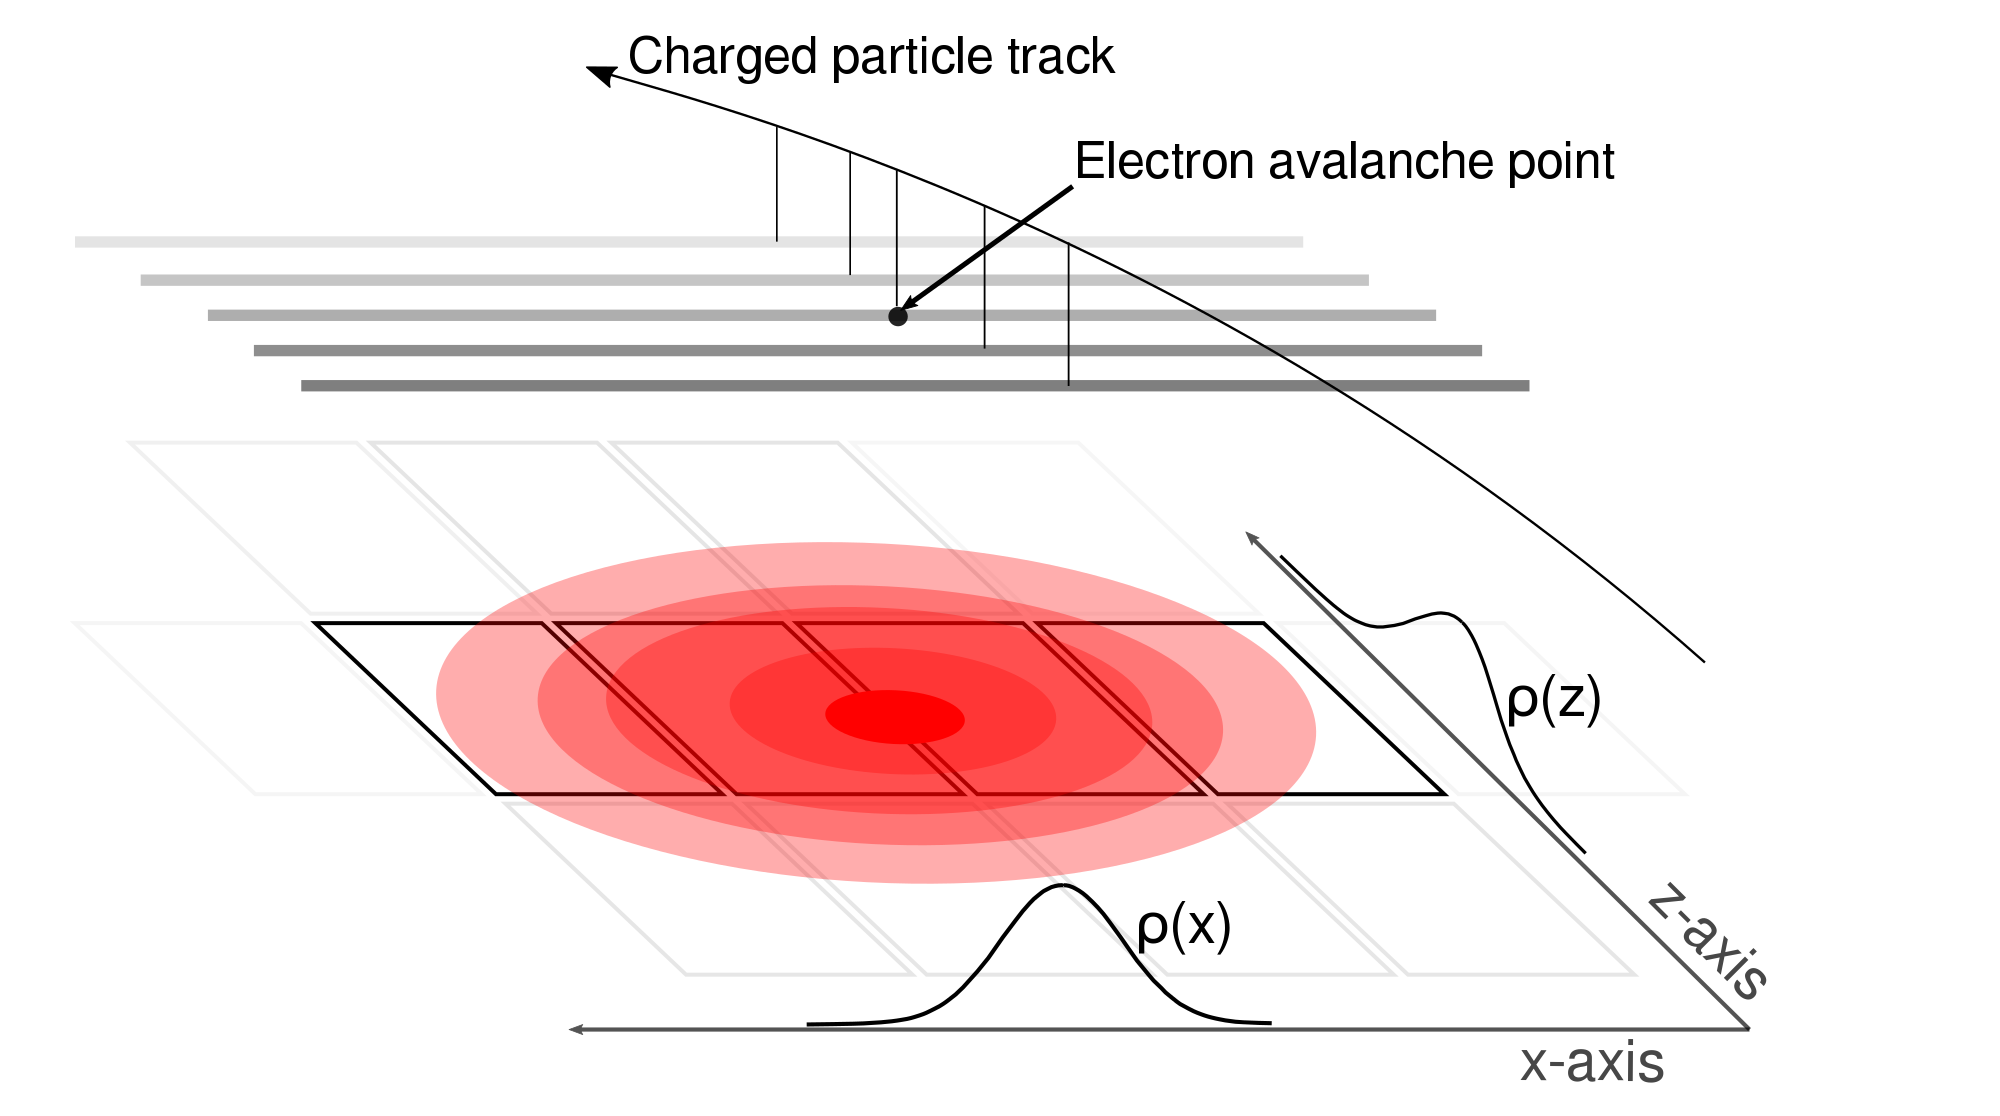
\includegraphics[width=\linewidth]{padsat_Large}
\caption{A cartoon illustration of the charge distribution resulting from an electron avalanche on one wire and the projections of the distribution onto the two axis $\rho(x)$ onto the x-axis and $\rho(z)$ onto the z-axis. The orientation of the wire planes is flipped upside down to display the perspective better.}
\label{fig:2DPRF}
\end{figure}

Gatti \cite{gatti} derived a semi-empirical formula for the charge distribution in a simple multi-wire TPC given as, 
\begin{equation}\label{eq:gatti}
\begin{split}
PRF_{\mathrm{Gatti}}(\lambda)
& = \frac{K_{1}}{K_{2}\sqrt{K_{3}}}\bigl[\arctan(\sqrt{K_{3}}\tanh\bigl[K_{2}\bigl(\frac{\lambda}{h}+\frac{w}{2h}\bigr)\bigr]) \\
& - \arctan(\sqrt{K_{3}}\tanh\bigl[K_{2}\bigl(\frac{\lambda}{h}-\frac{w}{2h}\bigr)\bigr])\bigr] \\
\end{split}
\end{equation}

where $w$ is the width of the pad, $h$ is the distance of the anode plane to the pad plane, and $\lambda$ is the distance of the pad center to the avalanche point. It is a single parameter equation where the two parameters $K_1 = \frac{K_{2}\sqrt{K_3}}{4 \arctan(\sqrt{K_3})}$ and $K_2 = \frac{\pi}{2}\left(1-\frac{\sqrt{K_{3}}}{2}\right)$ depend on the parameter $K_3$, which is a function of the ratio of the anode wire diameter to the distance of the anode wires to the pad plane. $K_3$ can be looked up in a graph in \cite{blumrol} and \cite{gatti}.


\begin{figure}[!htb]
\begin{overpic}[width=\linewidth]{fig5.pdf}
\put(61,55){\contour{white}{ PRF${}_{\mathrm{Gaus}}(\lambda)$ eq. \ref{eq:gaus}  }}
\put(61,49){\contour{white}{ PRF${}_{\mathrm{Gatti}}(\lambda)$ eq. \ref{eq:gatti} }}
\end{overpic}
\caption{Experimental pad response function of many events for a crossing angle of $85^{\circ} < \theta \leq 90^{\circ}$.  }
\label{fig:expprf}
\end{figure}


Since we take the marginal distributions only along one layer or row of pad  correlations are introduced in the PRF from adjacent layers or rows which cause slight deviations from the expected Gatti distribution. Also, analytic PRFs only exist for classical multi-wire TPCs. For these reasons it is useful to experimentally measure the PRF and fit it with an empirical function, typically a Gaussian, to describe its behavior. The method for extracting the experimental PRF will be discussed latter, by averaging over many events in the experimental data, the resulting PRF for the S$\pi$RIT TPC is shown in Fig.~\ref{fig:expprf}. Here we see the deviations from the expected analytic Gatti distribution (black curve), whereas fitting with a two parameter Gaussian function (red curve) gives a better description of the  data, Eq.~\ref{eq:gaus}, with the two parameters being the normalization coefficient, $N_0$, width $\sigma$, and with a mean value assumed to be 0.

\begin{equation}\label{eq:gaus}
PRF_{\mathrm{Gaus}}(\lambda) = N_0 e^\frac{-\lambda^2}{2\sigma^2}
\end{equation}





\begin{comment}
\subsection{Considerations when constructing a TPC}
Several considerations went into the construction of the S$\pi$RI TPC which I wish to summarize and document here. All materials and glues of the TPC were selected as low out-gassing materials. Several materials (that are common place in nuclear labs), such as vacuum grease, viton o-rings, all out-gas organic chemicals into the counter gas which damage the TPC by permanently lowering the gain over time. The organic molecules responsible are difficult to identify exactly, but lists of good and bad materials are well known in the literature from experiments. If a material we wished to used was not on these lists we placed the material in a clean chamber with the counter gas and flowed this counter gas through a small proportional counter making sure the gain did not drop at high collection rates when exposed to a high rate alpha Americium source. 

Sparking
Two volumes of gas. 
\end{comment}


\section{Radio Isotope Beam Factory (RIBF) Facility }
%Cyclotron facility overview.
%Samurai line overview.
%Beam line element overview.
%Big rips beam PID. reference 
The primary and secondary beams were produced at the Radioactive Isotope Beam Factory (RIFB) facility at RIKEN, in Wako-shi, Japan. The RIBF facility starts with two primary beam types, ${}^{132}$Xe and ${}^{238}$U, which produced by an ion-source and accelerated to progressively higher kinetic energies by 1 linear accelerator (RILAC), and 4 different cyclotrons (RRC, fRC, IRC, and SRC), reaching a primary beam energy of \SI{345}{\MeVA}. 



\begin{figure}[!htb]
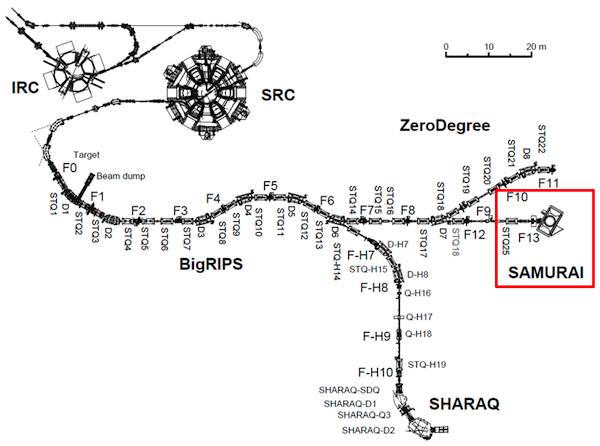
\includegraphics[width=\linewidth]{SAMURAI-beamline.png}
\caption{Overview of the RIBF, BigRIPS, and SAMURAI beamline.}
\label{fig:samuraiBeamLine}
\end{figure}

After the SCR, the primary beams impinge on a rotating \SI{3}{\milli\metre} Be target which produces many different species by fragmentation. These fragments are then separated by the BigRIPS spectrometer which is tuned to the particular secondary fragment of interest. This is accomplished through several dipole magnets, slits, and wedge degraders. The resulting secondary beam is not pure and the purity depends on the primary beam and target beam desired.

In these set of experiments several beams were produced with varying intensities and purities. Table~\ref{tb:beams} summarizes the average qualities of the 4 secondary beams produced in the two experimental campaigns. 

 \begin{table*}\centering
\ra{1.3}
\begin{tabular}{@{}ccccc@{}}\toprule 
 Primary Beam & Secondary Beam & Energy at mid target \si{\MeVA} & Intensity \si{\kilo\hertz} & Purity (\%) \\ [0.5ex] 
 \midrule
 ${}^{238}$U   & ${}^{132}$Sn   &  269.2  &  9.5  &  54   \\
 ${}^{238}$U   & ${}^{124}$Sn   &  270.3  &  9.1  &  10  \\
 ${}^{124}$Xe  & ${}^{112}$Sn   &  270.4  &  7.6  &  48  \\
 ${}^{124}$Xe  & ${}^{108}$Sn   &  269.3  &  7.5  &  52   \\
 \bottomrule
\end{tabular}
\caption{Primary and secondary beam properties produced in the \spirit TPC experimental campaigns. }
\label{tb:beams}
\end{table*}



\section{Experimental Setup}

The \spirit TPC was designed to fit exactly into the dipole gap of the  dipole magnet at the end of the BigRIPS beam line. Figure~\ref{fig:experiment} shows a drawing of the \spirit TPC inside of the SAMURAI magnet chamber which was rotated to the $\ang{0}$ configuration. Typically the SAMURAI (Superconducting Analyzer for Multi-particles from Radioisotope beams) is operated under vacuum as a large-acceptance multi-particle spectrometer for radioactive-beam experiments. This magnet can reach magnetic fields up to \SI{3}{\tesla} at the center of the pole gap. The space between the magnetic pole faces is further complicated by large bolts which protrude from the pole faces. These bolts secure the vacuum chamber to the magnet which is not practically removable; though the inside of the magnet was not operated under vacuum. This required an extensive rail system and support frame to slowly slide in the TPC over the bolts, finally raising the TPC several \si{\centi\metre} to the final height. 

\begin{figure}
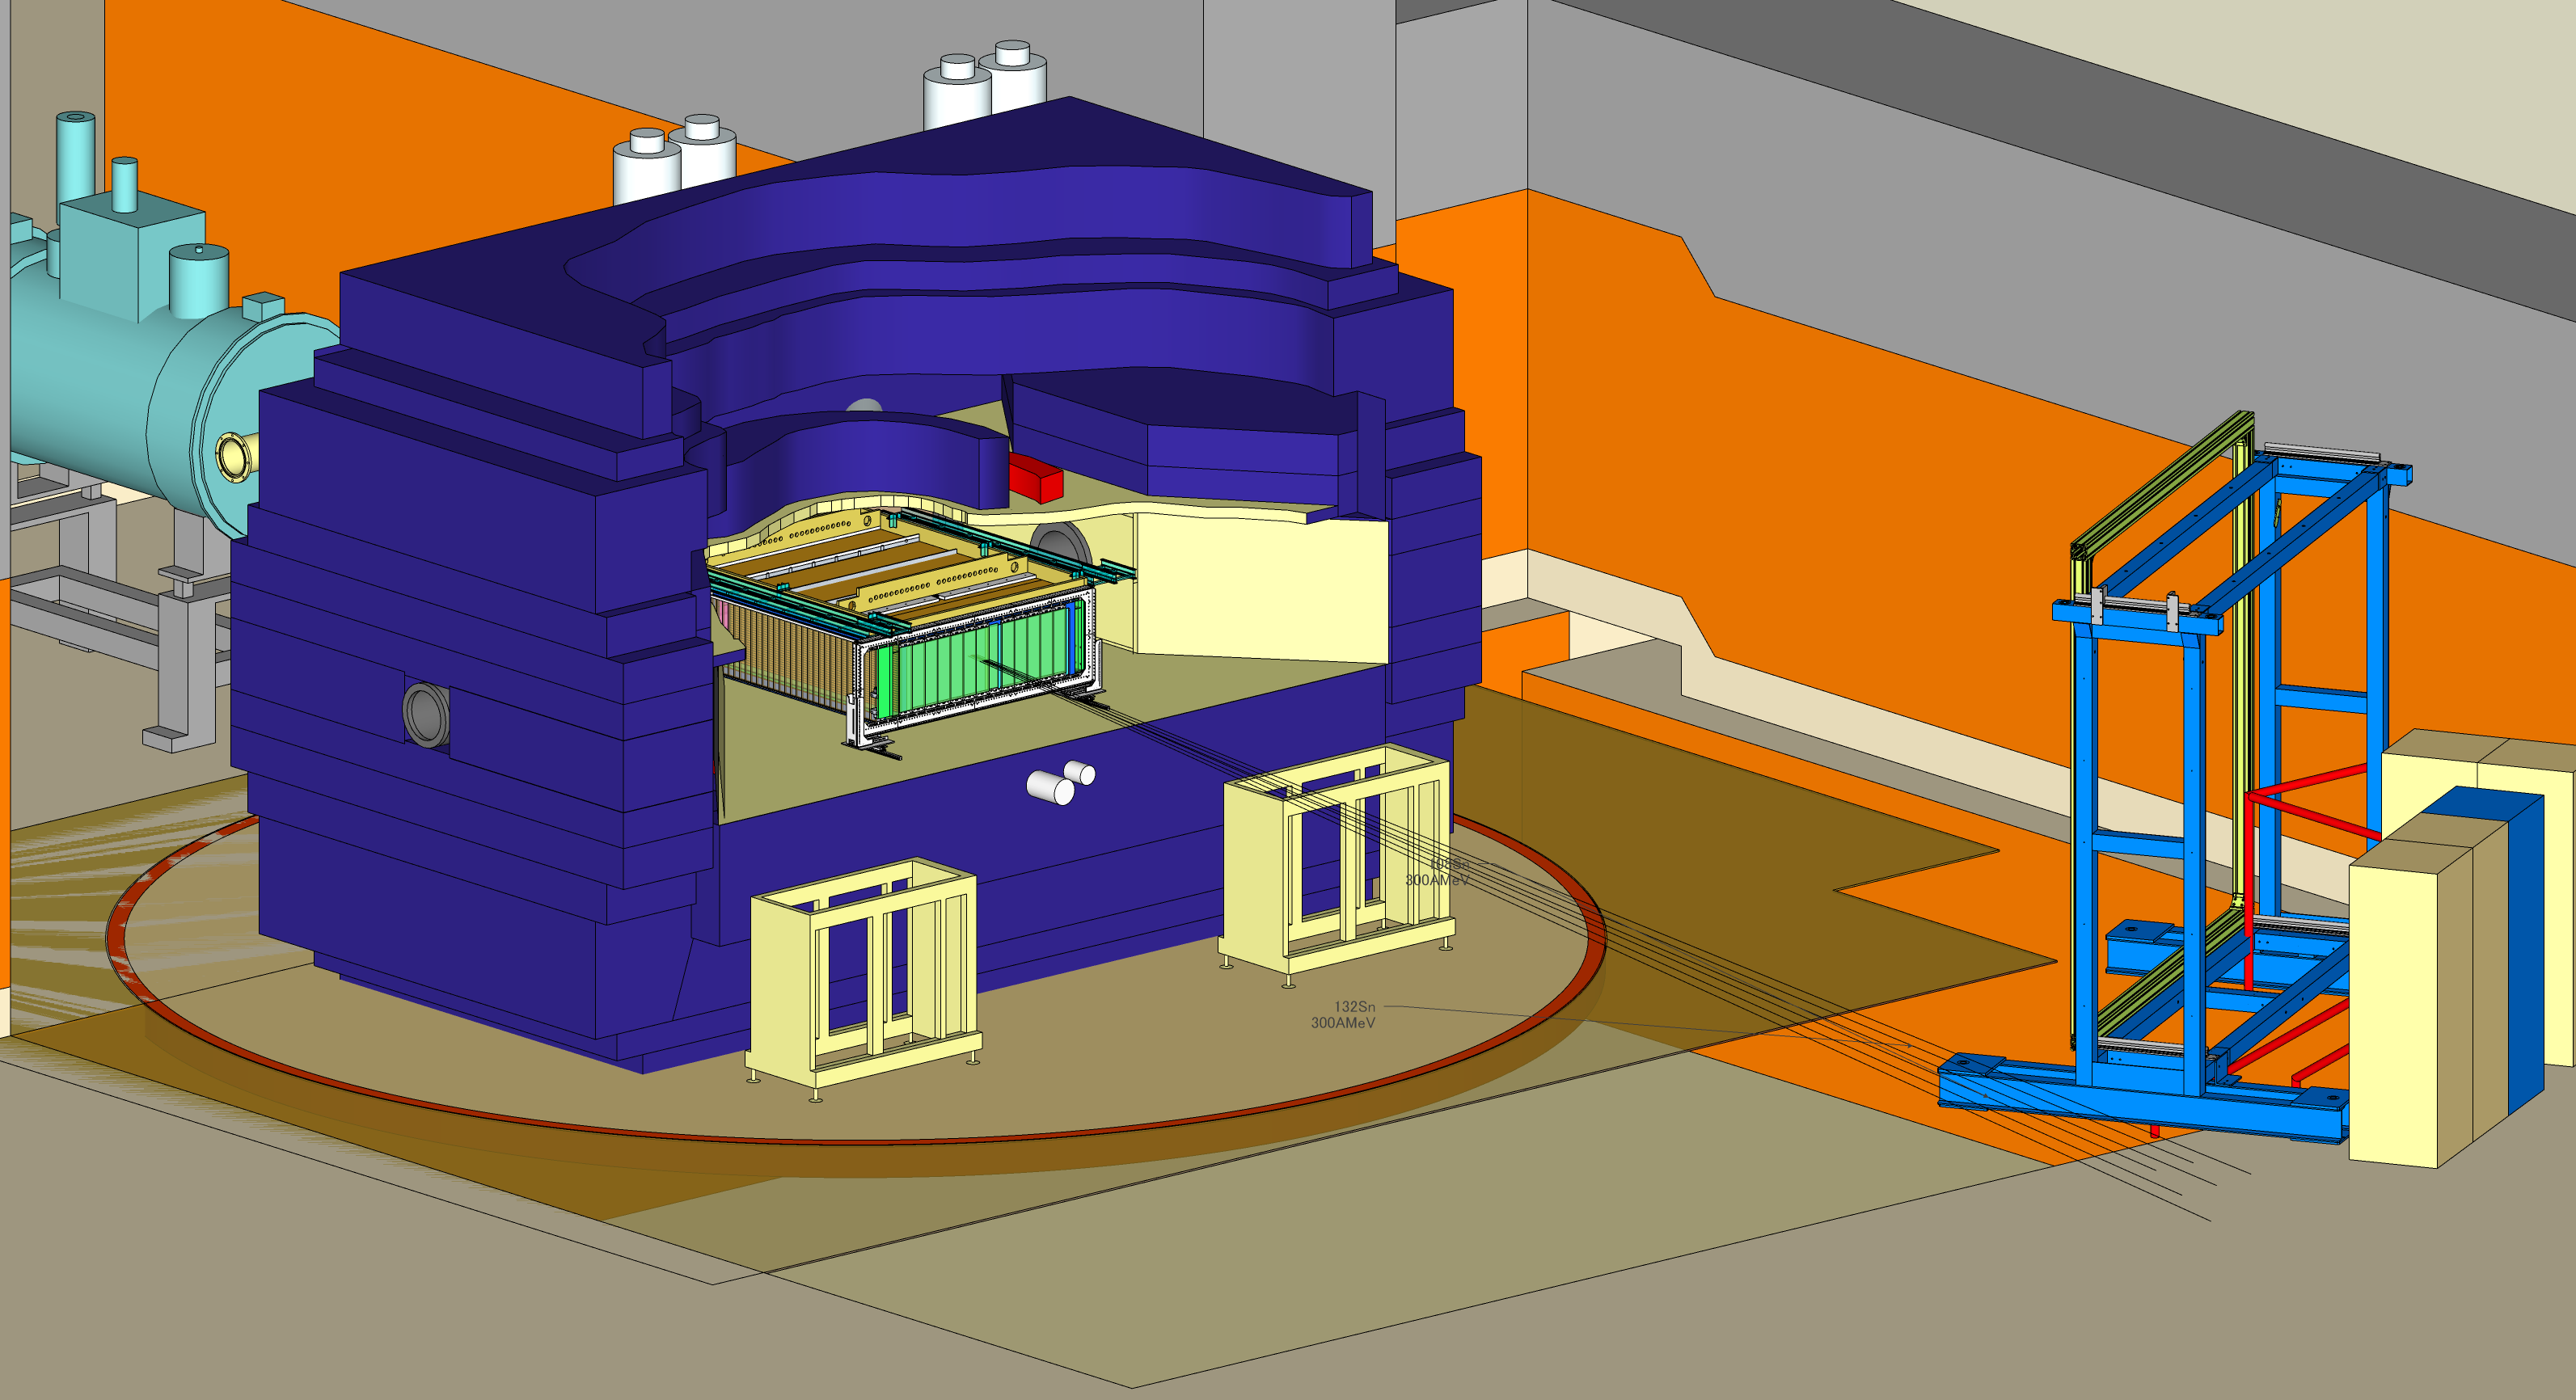
\includegraphics[width=\textwidth]{perspective.png}
\caption{Drawing of the experimental setup with the TPC inside of the SAMURAI magnet at $\ang{0}$ configuration.}
\label{fig:experiment}
\end{figure}

The height of the TPC was roughly aligned with a self-leveling laser system to match the center of target with the center of the beam line. Once the TPC was adjusted to the final location, the position of the TPC was measured in fine detail with a the VStars-N photogrametry system \cite{vstars}. Small highly reflective targets were placed all over the TPC both inside and out and pictures were taken with a calibrated lens and camera system. Using the commercial software provided the set of different camera perspectives reconstruct a point cloud of all the targets into 3-dimensional coordinates. Since the magnet was also measured with the same system after installation, we can match the two systems to get the absolute position of the TPC -- and several of its internal components-- relative to the magnet frame. The position resolution of this type of system was estimated to be around \SI{200}{\micro\metre} for each coordinate, which is much more precise than needed or Show data.

%Maybe put a position table summary here of the TPC position and definition of the coordinates system in the TPC frame and the Magnet frame


\section{Ancillary Detectors }
Several ancillary detectors were placed inside and outside of the \spirit TPC to facilitate making the trigger for the experiment. Placing detectors around the TPC was one of the important considerations we made when designing the TPC. A brief description of each detector system is given here with particular focus on how the experimental trigger was made. 

\subsection{Kyoto Multiplicity Trigger}
%kyoto array sets multiplicity trigger
%scintillator bars
The Kyoto Multiplicity Array consists of two arrays of plastic scintillating bars on each side of the TPC, each consisting of 30 bars. The entire TPC structure was designed so that light charged particles could easily pass through  the field cage and  side walls of the TPC enclosure. In this way the number of tracks passing through the sides of the TPC could be measured by this array. In heavy ion collisions the more central a nuclear collision is, the more nucleons participate in the collision, resulting in more measured tracks. It is this correlation between the number of tracks and centrality of the collision that makes the Kyoto Array sensitive to the centrality of events. It is more likely that in very central collisions more tracks are going to the peripheral angles and measured by the Kyoto array. In the experiment the trigger selection criteria was $n_{Kyoto} > 4$, where $n_{Kyoto}$ is the total number of tracks measured by both arrays. 

\begin{figure}[!htb]
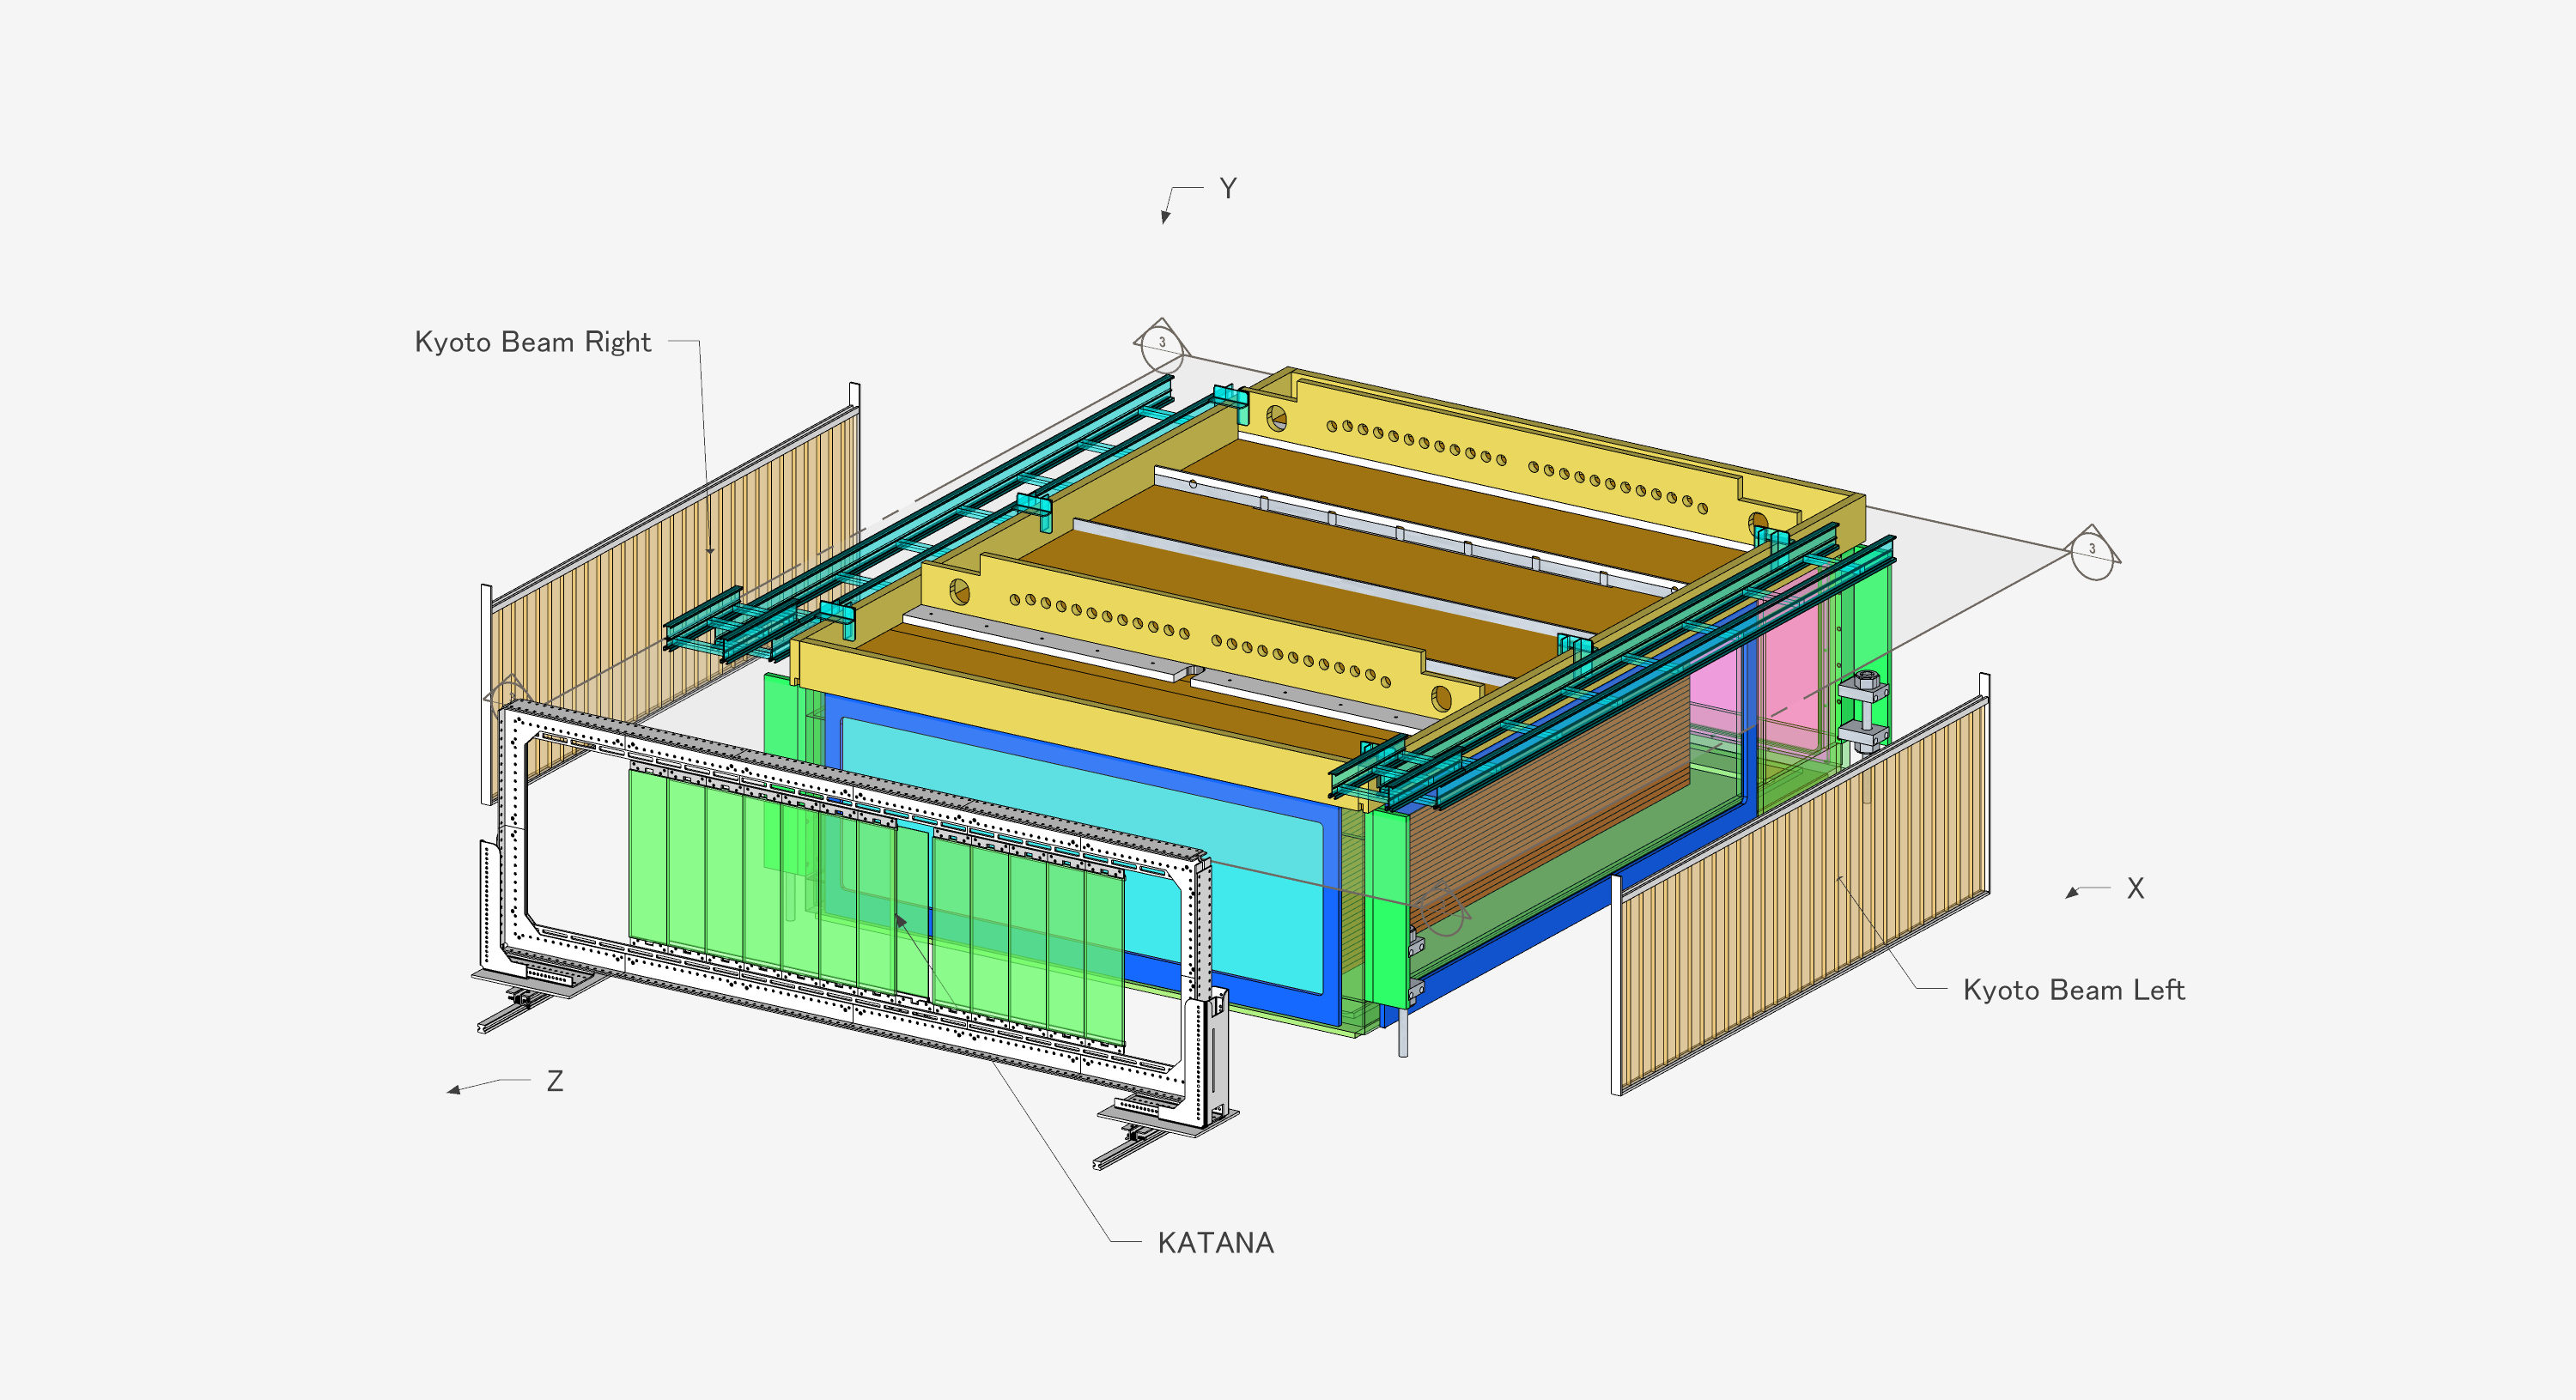
\includegraphics[width=\textwidth]{TPCAux.png}
\label{fig:aux}
\caption{Exploded views of Kyoto and KATANA arrays.}
\end{figure}


\subsection{Krakow KATANA Veto and Multiplicity Array}
%beam veto
%beam trigger optional
The Krakow KATANA array consists of 12 plastic scintillating bars mounted to the downstream wall of the TPC enclosure. Three of the 12 bars were thin and operated as a beam veto in the event the beam did not make a nuclear collision with the target; this was a majority of the time. The 9 other bars operated as an additional multiplicity array similar to the Kyoto array. Since most of the particles are focus forward in a cone in the laboratory frame, it was found the condition on the Kyoto array was sufficient to trigger on central events; thus the KATANA array was used in primarily the beam veto mode. This was accomplished by positioning the array so that the expected position of the beam exiting the TPC would be centered on the three thin paddles. The threshold of the veto paddles were set so that the charge of a particle, $Z$, was $Z > 20$. This allowed the selection of very central events and we did not trigger on very peripheral or no collision events. 


\subsection{Active Veto Array}
The beam was tuned by two sets of quadropole  magnets, STQ 1 and STQ2, so that the beam spot was focused on the TPC target location. Because of the inherent angular dispersion of the beam there were incoming beam events which significantly deviated from the target location. To veto these type of events an active veto array was set at the entrance of the TPC consisting of four small scintillating bars arranged to be slightly larger than the target size. The threshold was set so that any beam particle which passed through any of the bars it would send a trigger signal to not trigger the system since the beam path would not be on target but on some other material inside the TPC. 



\section{Data Acquisition (DAQ) }
The Data AcQuisition (DAQ) consisted of three different systems. The RIBFDAQ system served as the master DAQ for the BigRIPS beam identificaiton DAQ, the TPC DAQ, the NeuLAND neutron wall DAQ, and the Kyoto Array DAQ systems. The TPC DAQ was handled by the NARVAL framework to readout the GET electronics for the \spirit TPC. A General Trigger Operator (GTO) trigger was supplied to each DAQ synchronizing the subsystems. 

\section{Trigger Condition}
Signals from all of the auxiliary detectors were combined into several logic combinations to form a trigger logic for triggering the data acquisition  (DAQ) to record data. An upstream scintillating bar formed the start counter signal, triggering on any beam coming down the beam line. The active veto will trigger for any beam that is incident off the target location. The KATANA veto produces a signal if the beam passed through the TPC un-reacted, causing no nuclear collision; this produces a veto signal with a width of \SI{4}{\micro\second} which is the approximate time it takes for the beam to drift and clear the field cage volume. The Kyoto multiplicity trigger produces a signal when the total number of tracks passing through both Kyoto arrays are greater than 4. 


\begin{figure}[!htb]
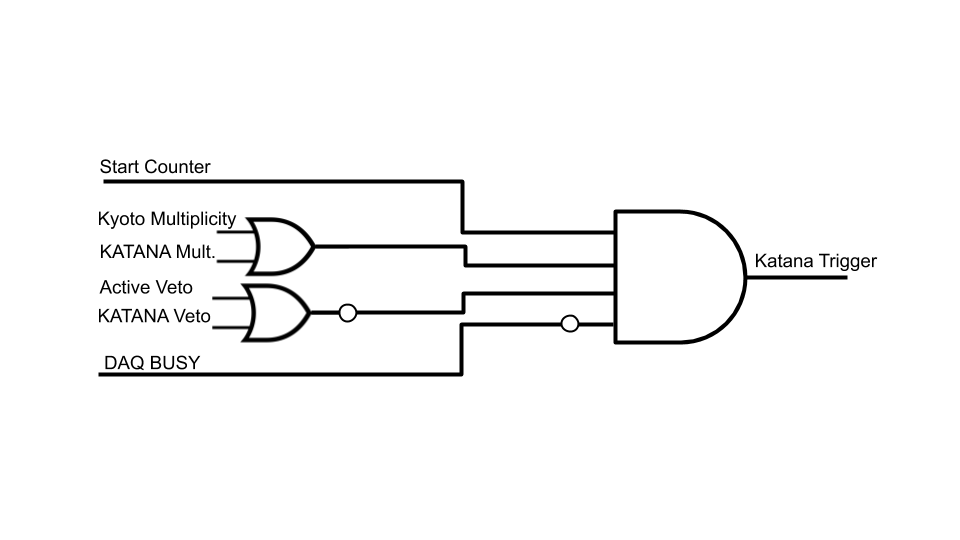
\includegraphics[width=\linewidth]{KatanaLogic.png}
\caption{KATANA trigger box logic.}
\label{fig:katanaLogic}
\end{figure}

\begin{figure}[!htb]
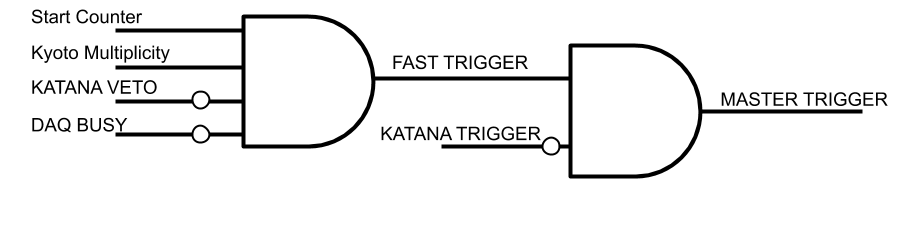
\includegraphics[width=\linewidth]{TriggerLogic.png} 
\caption{Master trigger logic.}
\label{fig:trigLogic} 
\end{figure}



\begin{figure}[!htb]
    \centering
    \begin{subfigure}[t]{0.45\textwidth}
        \centering
        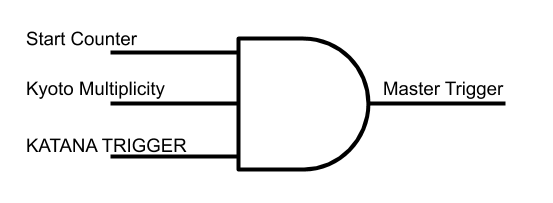
\includegraphics[width=\linewidth]{DataTrigger1.png} 
        \caption{${}^{124}$Xe primary beam trigger.} \label{fig:dataTrigger1}
    \end{subfigure}
    \hfill
    \begin{subfigure}[t]{0.45\textwidth}
        \centering
        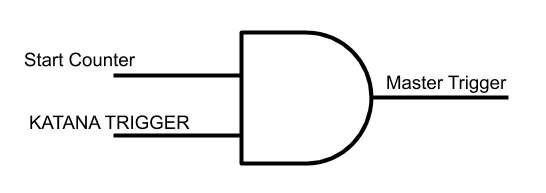
\includegraphics[width=\linewidth]{DataTrigger2.png} 
        \caption{${}^{238}$U primary beam trigger.} \label{fig:dataTrigger2}
    \end{subfigure}
\label{fig:datatrigger}
\end{figure}


There were several special trigger considerations when we built the trigger for the TPC. We required that the gating grid be opened fast to not miss any signal; as soon as there was a condition satisfying the Start Counter, Kyoto Multiplicity, the DAQ was not busy, and there was not a KATANA Veto signal. This was referred to as the Fast Trigger. If the KATANA trigger box is not satisfied --described later-- this will trigger a Fast Clear signal which will not trigger the DAQ and will quickly close the gating grid. Figure~\ref{fig:trigLogic} shows the logic of both of these triggers. 

The master trigger for the DAQ was different for each primary beam as the experiment got progressively better. During the ${}^{124}$Xe primary beam, the KATANA trigger box was an input into the trigger logic where as in the ${}^{238}$U primary beam, the KATANA trigger box functioned as the trigger logic utilizing the internal trigger electronics. In either case the differences in the trigger were very minor and they both behaved practically the same except for minor details on the gating grid trigger \cite{jon}. Figure~\ref{fig:katanaLogic} summarizes the KATANA trigger box logic. 

Figure~\ref{fig:dataTrigger1} summarizes the ${}^{132}$Xe primary beam, where the condition to produce a true KATANA trigger output was there must be a Start Counter, KATANA multiplicity, no Veto, and no DAQ busy signal. The KATANA trigger, Kyoto Muliplicity, and Start Counter together trigger the DAQ. 

 Where as Fig.~\ref{fig:dataTrigger2} summarizes the ${}^{132}$Xe primary beam, where the condition to produce a true KATANA trigger output was there must be a Start Counter, Kyoto or KATANA multiplicity, no Veto, and no DAQ busy signal. Here the KATANA trigger and the SC SUM??? togethere trigger the DAQ. 
 
 It is worth mentioning how the busy signals for the experiment were handled. The DAQ system itself produces a busy signal which was combined with the busy signals from either opening or closing the gating grid. When opening the gating grid it is assumed the full volume of the TPC will be read out and therefore  a \SI{11}{\micro\second} gate is produced; which is slightly more than the time it takes for all the electrons to drift in the field cage. In the case were the gating grid should be fast closed, either due to the fast clear circuit or the end of the TPC measurement, a \SI{5}{\micro\second} gate is produced to allow for the gating grid to settle to a closed configuration and clear the drift volume of any residual electrons from the beam. Both of these gates are included with the DAQ in an OR configuration which makes the overall busy signal. 
 


\section{Collision Data Taken}

